\chapterillustration{./abertura-ladrilhos}{./abertura-ladrilhos-professor}

\chapterwhat{Ladrilhamentos regulares, semirregulares e irregulares. }

\chapterbecause{O ladrilhamento de uma superfície plana é uma cobertura do plano onde formas (por exemplo, polígonos) são repetidos sem sobreposição ou buracos. No caso de polígonos, estes podem ser regulares ou não. Os ladrilhos compostos por figuras geométricas podem ser vistos como uma arte, usados em outras aplicações, como papéis de parede, forros de madeira, estamparia de tecidos, bordados entre outros. Apesar do número de possibilidades de realizar um ladrilhamento parecer infinita, é possível comprovar que ao utilizar apenas polígonos regulares existe apenas 11 possibilidades. Contudo pode-se aprofundar o estudo e investigar a utilização de polígonos irregulares.} 

\chapter{Ladrilhamento}
\label{ladri-chap}


%%%% Página de créditos

% Autores
\autorum{Carmen Vieira Mathias (UFSM)}
\autordois{Lucas Schimith Zanon (SEDUC - RS)}

% Revisores
\revisorum{José Ezequiel Soto}

\autordacapa{T.H. Chia}{Unsplash}{https://unsplash.com/photos/1-Zr2ye5588}
\versao{1.0}


\creditos

\mainmatter

\begin{apresentacao}{Introdução}
\subsection *{Habilidades e pré-requisitos}

Neste capítulo contempla-se a seguinte habilidade da versão homologada da Base Nacional Comum Curricular (BNCC) para o Ensino Médio:

\begin{habilities}{EM13MAT509}
Resolver problemas sobre ladrilhamento do plano, com ou sem apoio de aplicativos de geometria dinâmica, para conjecturar a respeito dos tipos ou composição de polígonos que podem ser utilizados em ladrilhamento, generalizando padrões observados.
\end{habilities}

 
As habilidades (conforme a versão homologada da BNCC para o Ensino Fundamental) consideradas como pré-requisitos para o entendimento dessa unidade são:

\begin{habilities}{EF03MA16}
Reconhecer figuras congruentes, usando sobreposição e desenhos em malhas quadriculadas ou triangulares, incluindo o uso de tecnologias digitais.
\tcbsubtitle{ EF05MA17} Reconhecer, nomear e comparar polígonos, considerando lados, vértices e ângulos, e desenhá-los, utilizando material de desenho ou tecnologias digitais.

\tcbsubtitle {EF06MA18} Reconhecer, nomear e comparar polígonos, considerando lados, vértices e ângulos, e classificá-los em regulares e não regulares, tanto em suas representações no plano como em faces de poliedros.
\tcbsubtitle {EF06MA19} Identificar características dos triângulos e classificá-los em relação às medidas dos lados e dos ângulos.
\tcbsubtitle {EF06MA20} Identificar características dos quadriláteros, classificá-los em relação a lados e a ângulos e reconhecer a inclusão e a intersecção de classes entre eles.
\tcbsubtitle {EF07MA27} Calcular medidas de ângulos internos de polígonos regulares, sem o uso de fórmulas, e estabelecer relações entre ângulos internos e externos de polígonos,
preferencialmente vinculadas à construção de mosaicos e de ladrilhamentos.

\tcbsubtitle {EF08MA18} Reconhecer e construir figuras obtidas por composições de transformações geométricas (translação, reflexão e rotação), com o uso de instrumentos de desenho ou de softwares de geometria dinâmica.
\end{habilities}




Considera-se também como pré-requisitos para o entendimento dessa unidade, as seguintes habilidades (conforme a versão homologada da BNCC para o Ensino Médio):
\begin{habilities}{EM13MAT105} 
Utilizar as noções de transformações isométricas (translação, reflexão,
rotação e composições destas) e transformações homotéticas para construir figuras e
analisar elementos da natureza e diferentes produções humanas (fractais, construções
civis, obras de arte, entre outras).
\end{habilities}

\subsection *{Tópicos abordados na unidade}
Nessa unidade serão abordados os seguintes assuntos:
\begin{itemize}
\item  Ladrilhamentos regulares, semirregulares e irregulares.
\item  O uso das isometrias na construção de ladrilhamentos.
\end{itemize}
	

Levando em consideração a habilidade EM13MAT509 citada anteriormente, os objetivos desse capítulo são:

\vspace{-1em}
\begin{itemize}
\item Reconhecer: 
\vspace{-.5em}
\begin{itemize}
\item os tipos de ladrilhamento do plano;
\item os possíveis ladrilhamentos do plano formado por polígonos regulares;
\item outros tipos de ladrilhamentos do plano.
\end{itemize}
\vspace{-.5em}
\item Explorar os conceitos geométricos necessários para a construção de ladrilhamentos do plano.
\end{itemize}
\vspace{-1em}


\subsection *{Abordagem adotada no capítulo}

Conforme mencionamos, a Base Comum Curricular (BNCC) – Brasil (2017) para o Ensino Fundamental (EF) aborda o tema ladrilhamento em uma das habilidades citadas, quando trata de polígonos, no sétimo ano.

\begin{habilities}{EF07MA22} Calcular medidas de ângulos internos de polígonos regulares, sem o uso de fórmulas, e estabelecer relações entre ângulos internos e externos de polígonos, preferencialmente vinculadas à construção de mosaicos e de ladrilhamentos, à confecção de ferramentas e peças mecânicas, entre outras. 
\end{habilities}

Os Parâmetros Curriculares Nacionais (PCN) (BRASIL, 1999) indicam o uso de ladrilhamentos como um procedimento para o cálculo de áreas.
\begin{quote}
Desse modo, o trabalho com áreas deve apoiar-se em procedimentos que favoreçam a compreensão das noções envolvidas, como obter a área pela composição e decomposição de figuras cuja área eles já sabem calcular (recortes e sobreposição de figuras) por procedimentos de contagem (papel quadriculado, ladrilhamento), por estimativas e aproximações (p.131).
\end{quote}

Brasil (1999) apresentam os ladrilhamentos, também para o EF no que tange o ensino de figuras geométricas.
\begin{quote}
No que diz respeito ao campo das figuras geométricas, inúmeras possibilidades de trabalho se colocam. Por exemplo, as atividades de classificação dessas figuras com base na observação de suas propriedades e regularidades. Atividades que exploram a composição e decomposição de figuras, como ladrilhamentos, tangrans, poliminós, fazem com que os alunos verifiquem que o recobrimento de uma superfície pode ser feito por determinadas figuras, como triângulos equiláteros, quadrados, retângulos, hexágonos regulares (p.123).
\end{quote}

Essa abordagem possui uma aproximação com o que a BNCC do o Ensino Médio (EM) apresenta para o campo da geometria. Observa-se que os ladrilhamentos não são citados nos PCN EM (Brasil, 2006), apesar da recomendação de trabalhar com padrões em sala de aula. 
\begin{quote}
[...] estimular a busca de regularidades, a generalização de padrões, a capacidade de argumentação, elementos fundamentais para o processo de formalização do conhecimento matemático e para o desenvolvimento de habilidades essenciais à leitura e interpretação da realidade e de outras áreas do conhecimento (p.42)
\end{quote}

Os padrões são importantes nesse contexto, pois, ladrilhamentos do plano são padrões repetidos de formas (geométricas ou não) denominadas ladrilhos. Essas formas devem preencher o plano sem lacunas e sem sobreposição (Billstein, Libeskind \& Lott, 2015). Também é importante que o ladrilhamento cubra  um plano infinito e isso será  possível, ao encontrar um padrão que se repete em todas as direções. Mesmo que uma forma cubra uma área ampla, não há um teste geral para saber se ela continuará a cobrir todo o plano (Eberle, 2014). Nesse contexto, no  presente capítulo, um ladrilhamento  será considerado como uma estrutura composta por uma área limitada que se repete em todas as direções. 

Acredita-se que um dos  objetivos ao propor o estudo de ladrilhamentos, principalmente nos anos iniciais da educação básica, deve ser melhorar as habilidades psicomotoras dos alunos e ensinar matemática com base em  atividades da vida diária, evoluindo do concreto ao abstrato. Além disso, artistas combinam matemática com arte e revelam a incrível beleza da geometria em áreas como têxteis, design de interiores, desenho industrial (Hatfieldet al, 2000). Além das preferências estéticas, os alunos precisam decidir quais formas são mais adequadas para preencher/decorar uma determinada área, levando em consideração as características das formas (Callingham, 2014). Pesquisas como Fuys, Geddes e Tischler(1988); Serra(1993) e  Wheatley e Reynolds(1996) mostram que trabalhar com ladrilhamentos do plano auxilia os alunos a compreender outros conceitos relacionados à geometria, como por exemplo áreas e transformações isométricas.  

Como ladrilhamento do plano é um conceito que pode melhorar a compreensão dos alunos sobre as concepções em geometria,  enquanto professores, podemos  solicitar aos alunos que expressem sua compreensão sobre os ladrilhamentos. Pois conforme Callingham(2004) concepções errôneas (missconceptions)  sobre esse assunto, podem afetar o desenvolvimento de outras ideias. Algumas pesquisas mostram que a maioria dos alunos do ensino fundamental apenas consegue descrever os ladrilhamentos de forma visual. Outras pesquisas apontam que os alunos podem fazer ladrilhamentos  usando objetos e formas geométricas desde a primeira série (Eberle, 2014; O'Daffer et al. 1998; Ward, 2003). Por outro lado, estudos como Outhred e Mitchelmore (2000) afirmam que as crianças não compreendem totalmente as sequências finitas de quadrados antes do quarto ou quinto ano. Marchini (2003) mostra que é  difícil para os alunos compreenderem a área infinita dos ladrilhamentos. Nessa pesquisa, o autor indica que os alunos pensam que o ladrilhamento está concluído quando o papel termina e o infinito não faz sentido. Além disso,  poucos alunos fazem tentativas criativas de adicionar um novo papel. Conforme Owens \& Outhred(1998) ao colocar ladrilhos em uma área limitada, os alunos trabalham mais com triângulos do que com retângulos. Isso indica que o sucesso dos alunos ao construir diferentes tipos de ladrilhamento  pode mudar.

Uma pesquisa muito interessante a respeito das dificuldades dos alunos sobre ladrilhamentos no plano é Callinghan (2004). Esse estudo focou em classificar a compreensão dos alunos sobre ladrilhamentos pelos níveis de pensamento geométrico de Van Hiele. Nesse contexto, no Nível 0 de acordo com os Níveis de Pensamento Geométrico de Van Hiele, esperava-se que os alunos reconhecessem as formas geométricas presentes no ladrilhamento, bem como a unidade fundamental ( forma ou combinação das formas) formam o padrão do ladrilhamento. No Nível 1, os alunos deveriam definir as formas e as transformçãoes  usadas para compor o ladrilhamento. No nível 2, espera-se que expliquem e façam alguma tentativa de medir a extensão da transformação, usando o nível de linguagem técnica, como “girar, rotacionar” ou “transladar ”. Embora o uso dos Níveis de Pensamento Geométrico de Van Hiele revele implicitamente os resultados acima mencionados, Callinghan (2004) sugere que a natureza dos equívocos que alguns alunos realizam não foi suficientemente definida por esta abordagem. 

Neste capitulo, não estamos interessando em identificar os Níveis de Pensamento Geométrico dos alunos, porém estes foram levados em conta ao pensarmos nas atividades propostas. Começamos trabalhando com ladrilhamentos monoédricos, formados por polígonos regulares e irregulares. Pensamos em começar por esse tipo de ladrilhamento, pois são mais simples de construir e por considerar que  os alunos estão familiarizados com a maioria das  formas. Os ladrilhamentos semirregulares que são os compostos por mais de um polígono regular, são trabalhados na sequencia. Após estudar e dominar esses conceitos, são propostas atividades onde os alunos necessitam utilizar conceitos de transformações isométricas para criar e explorar ladilhamentos.

Em todas as atividades do capítulo, pensamos em abordagens fundamentadas na metodologia de investigação matemática. Justifica-se essa escolha, pois conforme \cite[p.2]{Ponte} \textit{"em contextos de ensino, aprendizagem ou formação, investigar não significa necessariamente lidar com problemas na fronteira do conhecimento nem com problemas de grande dificuldade. Significa, apenas, trabalhar a partir questões que nos interessam e que se apresentam inicialmente confusas, mas que conseguimos clarificar e estudar de modo organizado." }

Além disso, pensamos que para aprender geometria, a investigação é um métodos eficazes de instrução. Nossa experiência didática mostra que os alunos, em geral, não conseguem aprender geometria por observação passiva, mas dão significado aos conceitos no momento que interagem com as formas. Dessa foram, em vários momentos, no decorrer do capítulo, serão propostas atividades com a utilização de materiais manipuláveis, para que os alunos possam investigar os conceitos por conta própria,  para determinar as propriedades em cada situação. 


\subsection *{Orientações sobre o uso do material}

Esse material é dividido em seções do tipo Explorando, Organizando, Praticando, Exercícios e Para saber mais. As seções explorando, organizando e praticando foram pensadas para o desenvolvimento em sala. As seções denominadas “\textit{Para saber mais}” são de caráter opcional, ao omiti-las não irá prejudicar o desenvolvimento das demais atividades. Apenas observamos que em geral  exploram aspectos interessantes do conteúdo. A seção denominada Exercícios contém atividades que devem ser desenvolvidos pelos estudantes fora do horário de aula. 

O material foi planejado para ser desenvolvido em 2 ou 3 semanas, em classes com três horas aula semanais e, para isso, seria necessário o desenvolvimento das atividades de modo eficiente pelos estudantes. Você  professor pode suprimir  algumas das atividades se julgar que a turma já possui nível de maturidade adequado naqueles tópicos


\end{apresentacao}

\def\currentcolor{session1}
\begin{texto}
{
	%\paragraph {Objetivos gerais da seção}

	%Reconhecer ladrilhamentos no plano

	\paragraph {Sugestões e discussões}
	Quando se trata de ladrilhamentos em matemática, também conhecidos como mosaicos ou pavimentações, é necessário explicar alguns termos comumente utilizados em outras áreas do conhecimento, caso esses apareçam na discussão.

	\begin{itemize}
	\item Ladrilho: laje de forma retangular ou quadrada, em geral de barro cozido.
	\item Azulejo: ladrilho vidrado em várias cores, mas que inicialmente era construído com a cor azul.
	\item Mosaico: conjunto embutido de pedras (pintadas ou não) com que se formam figuras ou desenhos.
	\item Mosaicista ou mosaísta: o que trabalha em obras de mosaico.
	\item Pavimentar: ato de recobrir artificialmente o chão ou o piso.
	\item Parquete: (do francês, parquet) pavimento construído com tacos de madeira, cerâmica ou outros materiais.
	\item Tecelagem: fábrica de tecidos, onde se tece.
	\item Tecelão: operário que lida com o tear, aparelho que tece, que faz o entrançamento dos fios. 
	\item Tessela: pedra para lajear, peça de mosaico.
	\item Tesselário: operário que prepara pedras para revestimento de pisos. (BARBOSA, 1993, p. 5).
	\end{itemize}

	Assim, pode-se considerar que mosaico é o resultado, é o produto final de uma pavimentação usando ou não algum tipo de padrão. Por sua vez, o termo tesselação é mais adequado para se referir a um padrão em tecidos, por exemplo. Quanto a ladrilhamento, é plausível concluir que são pavimentações construídas a partir de  polígonos regulares ou não.  Como foi colocado, propõe-se reconhecer ladrilhamentos no plano, assim, optou-se por utilizar preferencialmente esse termo. 
	No material disponibilizado ao estudante, ainda não faremos uma definição formal de ladrilhamento, porém utilizaremos a ideia que será utilizada é a seguinte: “Quando revestimos uma superfície plana com alguma figura sem deixar falhas ou sobrepô-las, dizemos que houve um ladrilhamento dessa superfície” (adaptado de BIANCHINI, 2015, p. 264).

}
\end{texto}
\clearmargin
\begin{objectives}{Brincando de ser Escher}
{
	\begin{itemize}
		\item Construir um ladrilhamento
		\item \textbf{Conceitos abordados}: ladrilhamentos de forma geral
	\end{itemize}	
}{1}{0}
\end{objectives}
\begin{sugestions}{Brincando de ser Escher}
{
	\textbf{Organização em sala de aula}: Nesta atividade, o aluno deve construir um ladrilhamento. O ideal é que ele faça isso individualmente. 

	\textbf{Dificuldades previstas}: É possível que inicialmente os alunos tenham alguma dificuldade, principalmente devido ao material utilizado. Mas a ideia é que os estudantes consigam montar o ladrilhamento usando as peças disponibilizadas.

	\textbf{Sugestões gerais}: Nesse momento espera-se que os alunos utilizem transformações no plano (de forma intuitiva) para que consigam construir o ladrilhamento utilizando o material proposto, analisem as imagens e percebam quais podem e quais não podem ser consideradas um ladrilhamento, justificando as suas respostas.

	Para o desenvolvimento da tarefa, recomenda-se : 
	\begin{itemize}
	\item Que o professor prepare o material com antecedência, imprimindo os lagartos do encarte em papel cartão, ou solicitando que os alunos o façam. 
	\item Caso o professor opte por utilizar o site indicado (\url{http://www.cdme.im-uff.mat.br/jogos_artisticos_geometricos_eletronico/Mosaico/aluno01.html}) , verifique se o mesmo está funcionando de forma satisfatória. 
	\item Caso tenha possibilidade de fazer a impressão dos elementos em impressora 3D, o Thingiverse possui alguns modelos prontos (\url{https://www.thingiverse.com/thing:89983}).
	\end{itemize}
 
	\textbf{Enriquecimento da discussão}: Sugere-se ainda que o professor incetive seus alunos a perceper quais as transformações os alunos utilizaram para construir o ladrilhamento. Recomenda-se que isso seja realizado enquanto os alunos tentam construir o ladrilhamento e em um momento posterior, quando os ladrilhamentos estiverem prontos.

	\textbf{Material necessário}: Lagartos impressos do encarte em folha de gramatura mais alta ou impressos em 3D .
}{0}{0}
\end{sugestions}
\begin{objectives}{Reconhecendo um ladrilhamento}
{
	\begin{itemize}
	\item Reconhecer um ladrilhamento
	\item \textbf{Conceitos abordados}: ladrilhamentos de forma geral.
	\end{itemize}
}{1}{0}
\end{objectives}
\begin{sugestions}{Reconhecendo um ladrilhamento}
{
	\textbf{Organização em sala de aula}: Nesta atividade, inicialmente o aluno deve verificar se determinada figura é ou não um ladrilhamento. O ideal é que ele faça isso individualmente e depois compartilhe em pequenos grupos. Em um momento posterior, faz-se a discussão no grande grupo.

	\textbf{Dificuldades previstas}: É possível que inicialmente os alunos tenham alguma dificuldade, visto que é um conceito novo e visto que os exemplos colocados servem exatamente para gerar discussão e questionamentos. 

	\textbf{Sugestões gerais}: Nesse momento espera-se que os alunos analisem as imagens e percebam quais podem e quais não podem ser consideradas um ladrilhamento, justificando as suas respostas.

	Para o desenvolvimento da tarefa, recomenda-se que: 
	\begin{itemize}
	\item O professor apresente outros exemplos, ou solicite que os alunos pesquisem com antecedência ( Parte 2: Onde podemos encontrar ladrilhamentos no mundo ao nosso redor? Vamos pensar em alguns exemplos?).
	\item Depois que os alunos apresentaram seus exemplos, o professor pode projetá-los(com o auxílio de um projetor multimídia) incentivando a autonomia e protagonismo dos estudantes. 
	\end{itemize}
}{1}{0}
\end{sugestions}
\begin{answer}{Reconhecendo um ladrilhamento}
{
	O objetivo da atividade Reconhecendo um ladrilhamento é fazer com que os alunos consigam definir ladrilhamento a partir dos exemplos apresentados. São expostas 6 figuras, cuja intenção é provocar discussão.

	\textbf{Figura 1}- A ilustração representa uma "pavimentação" de peças de um quebra-cabeça monocromático, em que algumas peças estão sobrepostas e  existem  espaços não utilizados (lacunas).  Os "ladrilhos" deveriam se encaixar montando o quebra-cabeça. Além disso, não existe um padrão sendo respeitado. Então “NÃO”

	\textbf{Figura 2}- As formas se repetem perfeitamente, sem espaços ou sobreposições, logo a resposta é SIM, pois em um ladrilhamento do plano, as formas devem se encaixar, sem espaços ou sobreposições.

	\textbf{Figura 3} - A forma básica (papéis adesivos no formato quadrado) se repete de forma desordenada  em que algumas peças estão sobrepostas e  existem  espaços não utilizados (lacunas). 

	\textbf{Figura 4} - A forma básica (papéis recortados no formato de círculos) se repete. Apesar de parecer existir um tipo de ordem na posição das formas, existem espaços não utilizados.

	\textbf{Figura 5}- Na metade inferior esquerda da foto, sim porque as penas se encaixam sem folgas ou sobreposições e claramente, esse padrão pode ser repetido para sempre para preencher um plano. No entanto, na metade superior direita da foto, muitas das penas estão sobrepostas. Os "ladrilhos" em não devem se sobrepor. Então, na área superior direita, "NÃO"

	\textbf{Figura 6}-  As formas se encaixam, se repetem perfeitamente e não existe sobreposições. logo a resposta é SIM.
}{0}
\end{answer}


\explore{A arte de ladrilhar}
\label{ladri-exp-1}

Devido às suas características e sua estética decorativa, os ladrilhamentos foram utilizados tanto na arte quanto na arquitetura, fornecendo revestimentos para paredes, calçadas e tetos de muitas instalações. 

A origem dos ladrilhamentos ocorreu a cerca de  4.000 anos, quando os sumérios usavam azulejos de barro para compor elementos de decoração em suas casas e templos. A partir daí, o ladrilhamento encontrou seu lugar em elementos artísticos de muitas civilizações. 

No século XIX, intelectuais começaram a observar os ladrilhamentos presentes na natureza, a fim de explicar suas estruturas geométricas, o que resultou em numerosos estudos baseados em matemática. Um exemplo é  o artista Maurits Escher que usou o conceito de ladrilhamento para criar obras de arte. Esse artista holandês era fascinado por ladrilhamentos, também chamados de pavimentações ou mosaicos. 

Escher fez alguns ladrilhamentos enigmáticos, começando com uma forma básica e depois transformando-a usando isometrias.  Tais obras são muito complexas e em muitas delas aparecem formas de  animais e humanos, como por exemplo na obra  Lizard (lagartos) criada em 1942, ilustrada na \hyperref[lad-fig-1]{figura \ref{lad-fig-1}}.

\begin{figure}[H]
\centering
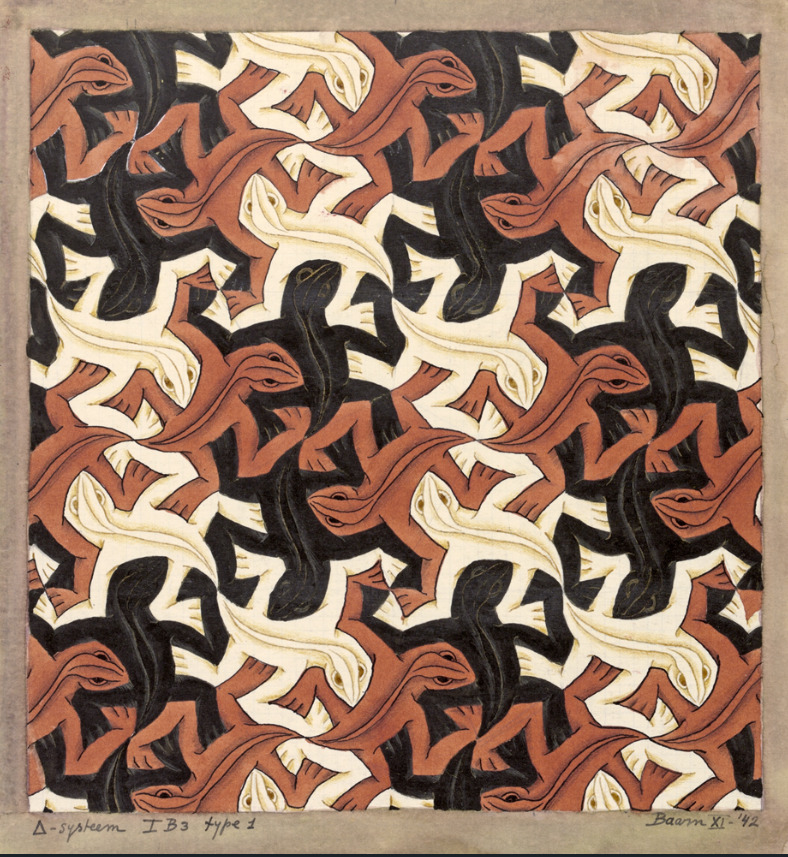
\includegraphics[width=200bp]{lagartos}

\caption{Lizard, M.C. Escher. Fonte: \href{https://www.wikiart.org/en/m-c-escher/lizard-1}{Wikiart}}
\label{lad-fig-1}
\end{figure}


Mas, um ladrilhamento nem sempre cobre uma superfície plana. Por exemplo, essa  superfície pode ser a parte externa de uma bola ou de um abajur. Pode ser  a parte interna de um ovo decorado, a pele de uma cobra, um hexágono plano ou uma parede. Assim, neste capítulo, vamos reconhecer, descrever e criar ladrilhamentos, para explorar e percebê-los no ambiente que nos cerca.

\begin{reflection}
Escher criou o ladrilhamento ilustrado na \hyperref[lizard]{figura \ref{lizard}}  transformando um hexágono em um lagarto. Como será que ele fez isso?
\end{reflection}



\begin{task}{Brincando de ser Escher} \label{at_brinc}
Será que os lagartos (\hyperref[lizard]{figura \ref{lizard}}) podem ser usados para ladrilhar o plano? 
Utilize o material disponibilizado por seu professor para construir o ladrilhamento.


\begin{figure}[H]
\centering
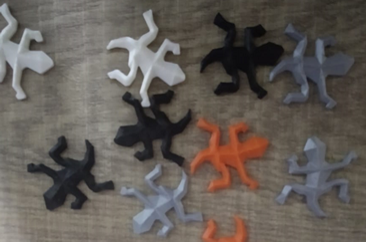
\includegraphics[width=290bp]{ladrilhamento3}
\caption{Lagartos}
\label{lizard}
\end{figure}
\end{task}


\begin{task}{Reconhecendo um ladrilhamento} \label{rec_lad}
\begin{enumerate}
\item Considere  a \hyperref[ladr12]{figura \ref{ladr12}}, composta de seis outras imagens. Decida se as imagens (numeradas de 1 a 6) podem ou não podem ser  ladrilhamento.

\begin{figure}[H]
\centering
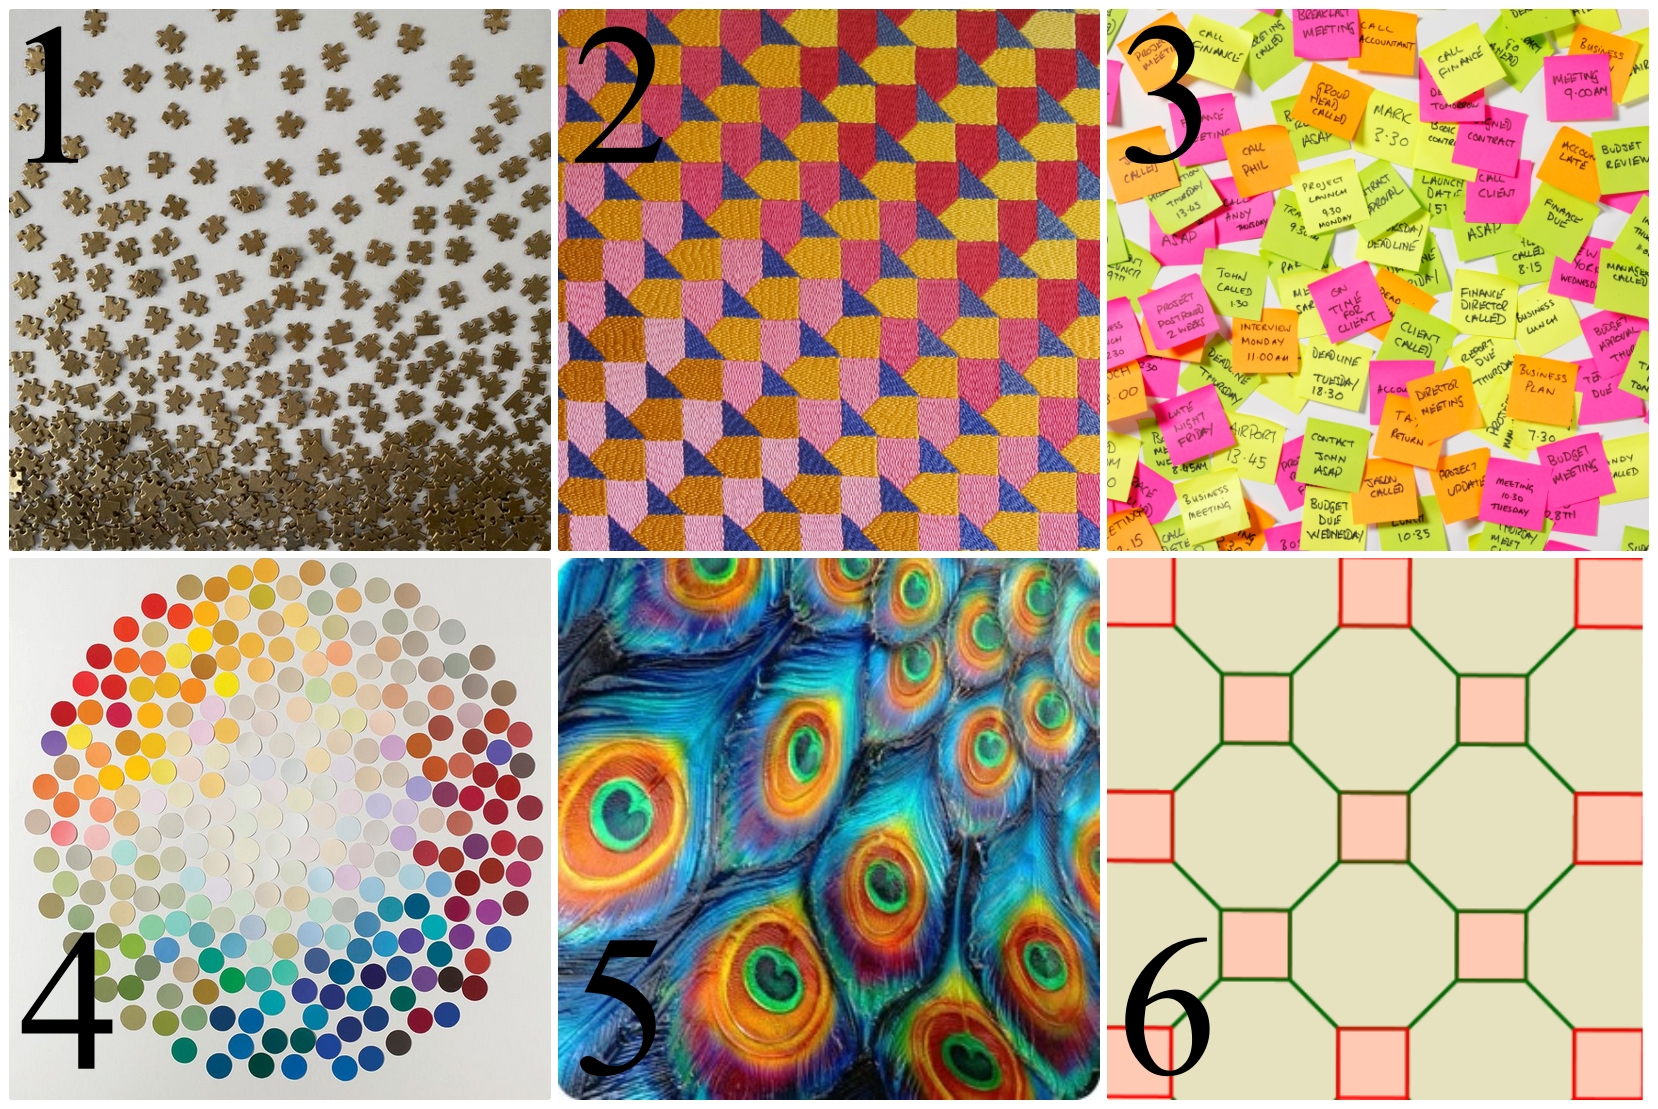
\includegraphics[width=300bp]{reviso1}
\caption{Imagens que podem ilustrar ladrilhamentos.}
\label{ladr12}
\end{figure}

\item Onde podemos encontrar ladrilhamentos no mundo ao nosso redor? Cite alguns exemplos?

\end{enumerate}

\end{task}



\arrange{A arte de ladrilhar}

No primeiro item da \hyperref[rec_lad]{atividade \ref{rec_lad}} nosso objetivo foi que você identificasse quais das imagens eram ladrilhamentos.
Observamos que as figuras 1, 3, 4 e 5 não são ladrilhamentos, visto que os requisitos:  obedecer um padrão, não existir espaços não utilizados (lacunas) e não haver sobreposição de formas, não são cumpridos. A figura 5 (penas do pássaro) parece obedecer essas condições, pois na metade inferior esquerda da foto, as penas se encaixam sem folgas ou sobreposições e claramente, esse padrão pode ser repetido para sempre para preencher um plano. No entanto, na metade superior direita da foto, muitas das penas estão sobrepostas. E como os "ladrilhos" não devem se sobrepor. Então, a figura não é um ladrilhamento.

Assim, as figuras em que as formas se repetem perfeitamente, sem espaços ou sobreposições, podendo ser repetidas indefinidamente são as figura 2 e 6.
Assim,  quando revestimos uma superfície plana com figuras sem deixar falhas ou sobrepô-las, dizemos que houve um ladrilhamento dessa superfície. 

No segundo item parte da  \hyperref[rec_lad]{atividade \ref{rec_lad}} questionamos onde é possível encontrar encontrar ladrilhamentos no mundo ao nosso redor. 
Ao observarmos a natureza, um dos exemplos mais conhecidos de ladrilhamentos são os favos de mel, que são formas tridimensionais hexagonais. Pode-se observar que não há lacunas entre as formas. Sem lacunas, as abelhas usam seu espaço de armazenamento de forma muito eficiente. Outros exemplos são as peles de algumas cobras e o pelo da girafa (\hyperref[natureza]{figura \ref{natureza}}).


\begin{figure}[H]
\centering
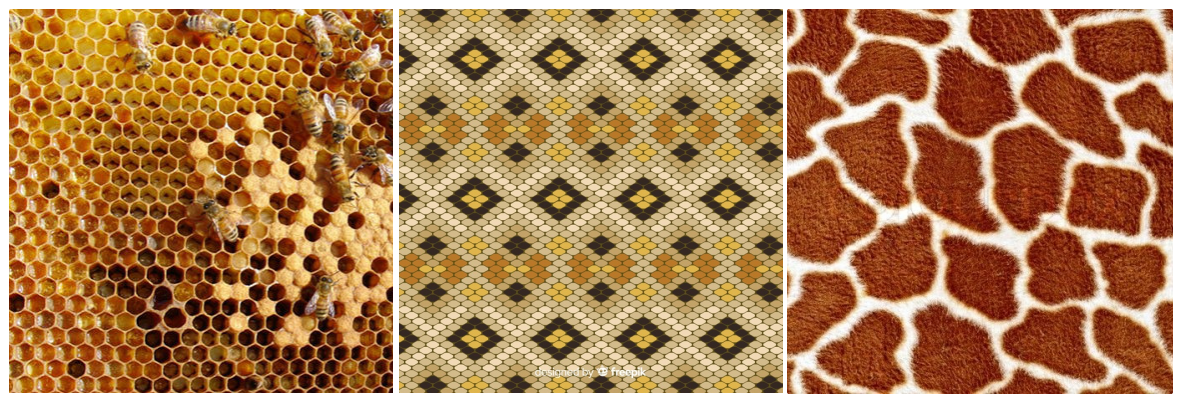
\includegraphics[width=400bp]{reviso2}
\caption{Ladrilhamentos na natureza. Fonte: Google Imagens}
\label{natureza}
\end{figure}

Também é possível perceber a presença de ladrilhamentos do plano no revestimento de pisos e paredes (\hyperref[natureza1]{figura \ref{natureza1}}). 


\begin{figure}[H]
\centering
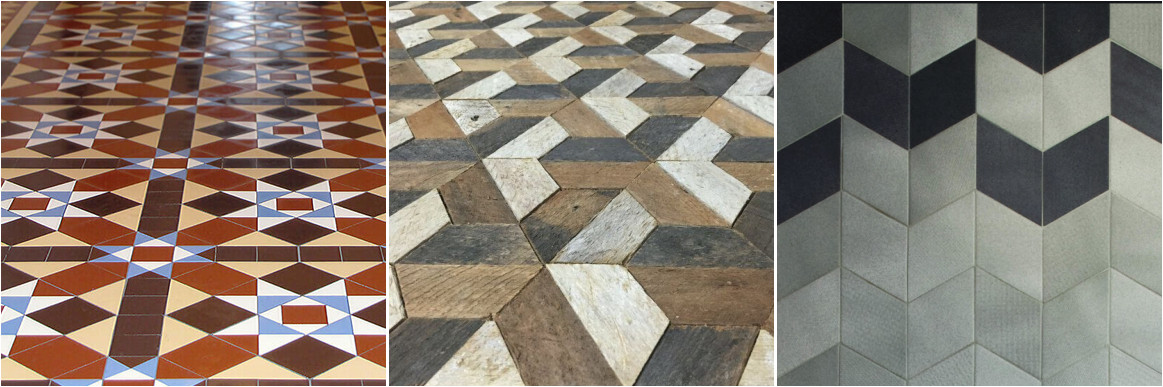
\includegraphics[width=400bp]{nature3}
\caption{Revestimento de pisos e paredes. Fonte: Google Imagens}
\label{natureza1}
\end{figure}

Um dos objetivos desse capítulo é que você construa alguns ladrilhamentos, e para começar, foi proposta a \hyperref[at_brinc]{atividade \ref{at_brinc}}. Foi possível construir um ladrilhamento usando apenas lagartos?  Mas o que os lagartos tem em comum com a matemática? 

Os ladrilhamentos têm sido amplamente utilizados na arte e na arquitetura desde os tempos antigos, mas o que existe associado a isso é  matemática. A teoria é extensa, mas explicaremos alguns princípios básicos para nos aproximar do que está por trás de belas obras de arte. 

Quando se trata de ladrilhamento em matemática, também conhecido como mosaico ou pavimentação, é necessário explicar vários termos técnicos com os quais a geometria opera. Por exemplo, uma forma fundamental (também chamado de ladrilho) é uma peça que é repetida para formar um ladrilhamento. Na atividade anterior, a peça que foi repetida foi o lagarto.


No caso da matemática, geralmente, trabalha-se com polígonos e nesse caso é necessário observar que ao revestimos uma superfície plana com um ou mais polígonos, não devemos  deixar falhas ou fazer sobreposições e é sobre isso que tratará a próxima seção.


\know{Tesselação} \label{tess}

Tesselação é outra palavra para ladrilhamento. Derivado da palavra latina, tessella, que eram os pequenos pedaços de pedra usados para fazer mosaicos romanos, uma tesselação ou ladrilho, é um padrão feito de uma ou mais formas que se encaixam sem lacunas ou sobreposições.
Destas palavras antigas derivam termos semelhantes que aparecem em várias aplicações práticas, da arte e arquitetura à ciência, tecnologia e produção.

Em design e arquitetura, a tesselação se refere à pavimentação de paredes, pisos ou outras superfícies com um padrão de pequenos ladrilhos feitos de cerâmica, vidro ou outros materiais. Esses ladrilhos normalmente são cortadas em formas geométricas que se encaixam perfeitamente em designs simples ou complexos formando um padrão aparentemente infinito. A aplicação de ladrilhamentos  na arquitetura  é  amplamente encontrada em muitas civilizações do mundo, incluindo o antigo Egito, Pérsia, Arábia, Japão e China, existindo ao longo da história do desenvolvimento da arquitetura. Embora os ladrilhamentos geralmente consistam em formas abstratas, principalmente retângulos, hexágonos, octógonos e outros polígonos, também podem consistir em elementos figurativos, como no trabalho de artistas como M.C. Escher (1898-1972). Escher é famoso por suas tesselações compostas de cavalos, borboletas, pássaros e criaturas imaginárias.


\clearpage
\def\currentcolor{session1}
\begin{texto}
{
	%\paragraph {Objetivos gerais da seção}
	%\begin{itemize}
	%\item Criar ladrilhamentos do plano, usando apenas um tipo de polígono regular.
	%\item Reconhecer quais polígonos regulares ladrilham o plano.
	%\item Reconhecer que alguns polígonos irregulares ladrilham o plano.
	%\end{itemize}


	Observamos que todas as atividades desse explorando são muito parecidas, porém cada uma tem um objetivo específico.

	\paragraph {Sugestões e discussões}

	Uma pergunta que deve ser respondida no decorrer dessa seção é: quais polígonos regulares pavimentam o plano. No livro do aluno essa resposta não será imediata, pretende-se que os alunos investiguem, por meio de experimentação, feita com materiais manipuláveis ( polígonos regulares congruentes recortados em cartolina ou em EVA, cortados a laser ou impressos em 3D) ou por meio de aplicativos a resposta ao questionamento. Dessa forma, em todas as atividades dessa seção, o professor poderá optar pela Parte 1 ou pela Parte 2, caso tenha pouco tempo para explorar o tema. No organizando haverá a formalização do que foi abordado.  
}
\end{texto}
\begin{objectives}{Ladrilhamento usando triângulos}
{
	\begin{itemize}
	\item Criar Ladrilhamentos do plano usando apenas um tipo de triângulo (equilátero ou não).
	\item Reconhecer que qualquer triângulo ladrilha o plano.
	\item \textbf{Conceitos abordados}: Ladrilhamenos monoédricos.
	\end{itemize}
}{1}{1}
\end{objectives}
\begin{sugestions}{Ladrilhamento usando triângulos}
{
\textbf{Organização em sala de aula}: Sugerimos que as atividades sejam realizadas de forma individual ou em duplas. A reflexão mediada pela manipulação dos polígonos pode ser favorecida pela discussão com um colega. Grupos maiores podem gerar dispersão.

\textbf{Dificuldades previstas}: É possível que inicialmente os alunos tenham alguma dificuldade, principalmente devido ao material utilizado (ou os aplicativos ou o material manipulativo). Mas a ideia é que os estudantes consigam montar o ladrilhamento usando as peças disponibilizadas.  Observar que os alunos podem construir pavimentações como a seguinte:

\begin{figure}[H]
\centering

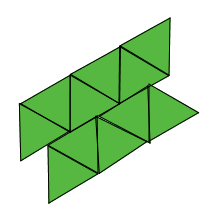
\includegraphics[width=150bp]{ladrilhamento-professor1}
\end{figure}

\begin{itemize}
\item Que não ladrilhamentos que satisfazer a condição: "Para isso, procure distribuir os triângulos ao redor de um vértice". Mas será salutar que isso ocorra, para que o aluno perceba a condição imposta e não repita o "erro" nas demais atividades.
\end{itemize}

\textbf{Enriquecimento da discussão}: Sugere-se que o professor incentive seus alunos a perceber quais as transformações isométricas utilizaram para construir o ladrilhamento. Recomenda-se que isso seja realizado enquanto os alunos tentam construir o ladrilhamento e em um momento posterior, quando os ladrilhamentos estiverem prontos.

\textbf{Material necessário}: Polígonos impressos do encarte em folha de gramatura mais alta, recortados em EVA, feitos com MDF em corte a laser ou impressos em 3D e aplicativos indicados .

}{0}{0}
\end{sugestions}
\begin{answer}{Ladrilhamento usando triângulos}
{
	\begin{enumerate}
	\item ---
	\item ---
	\item Primeiro ladrilhamento continha um triângulo com lados iguais, já o segundo com lados diferentes entre si.
	\item 
	\begin{enumerate}
	    \item Sim.
		\item Sim, todo triângulo pode ladrilhar um plano. O triângulo irregular é aquele que não possui.
		\item Serão congruentes quando satisfizerem um dos condições de congruência, por exemplo, lados correspondentes congruentes
		\item Sim, pela “regra imposta”: procure distribuir os triângulos ao redor de um vértice.
		\item  Por exemplo,  usou translações, rotações ou reflexões ou uma combinação de transformações
	\end{enumerate}
	\end{enumerate}
}{0}
\end{answer}
\clearmargin
\begin{objectives}{Ladrilhamentos usando quadriláteros}
{\begin{itemize}
	\item Criar ladrilhamentos do plano usando apenas um tipo de quadrilátero.
	\item Reconhecer que todos os quadriláteros ladrilham o plano.
	\item \textbf{Conceitos abordados}: Ladrilhamentos monoédricos.
\end{itemize}
}{1}{0}
\end{objectives}
\begin{sugestions}{Ladrilhamento usando quadriláteros}
{
\textbf{Organização em sala de aula}: Sugerimos que as atividades sejam realizadas de forma individual ou em duplas. A reflexão mediada pela manipulação dos polígonos pode ser favorecida pela discussão com um colega. Grupos maiores podem gerar dispersão.

\textbf{Dificuldades previstas}: É possível que inicialmente os alunos tenham alguma dificuldade, principalmente devido ao material utilizado (ou os aplicativos ou o material manipulativo). Mas a ideia é que os estudantes consigam montar o ladrilhamento usando as peças. 

\textbf{Sugestões gerais}: Uma pergunta que deve ser respondida no decorrer dessa seção é: quais polígonos regulares pavimentam o plano. No livro do aluno essa resposta não será imediata, pretende-se que os alunos investiguem, por meio de experimentação, feita com materiais manipuláveis ( polígonos regulares congruentes recortados em cartolina ou em EVA, cortados a laser ou impressos em 3D) a resposta ao questionamento. No organizando haverá a formalização do que foi abordado.  Os alunos podem ter dificuldade com o conceito de convexo. Pode ser necessário uma explicação para o conceito. 

\textbf{Enriquecimento da discussão}: Sugere-se que o professor incentive seus alunos a perceber quais as transformações utilizaram para construir o ladrilhamento. Recomenda-se que isso seja realizado enquanto os alunos tentam construir o ladrilhamento e em um momento posterior, quando os ladrilhamentos estiverem prontos.

\textbf{Material necessário}: polígonos impressos do encarte em folha de gramatura mais alta, recortados em EVA, feitos com MDF em corte a laser ou impressos em 3D e aplicativos indicados .
}{0}{0}
\end{sugestions}
\begin{objectives}{Ladrilhamento usando pentágonos}
{
\begin{itemize}
\item Reconhecer que os pentágonos regulares não ladrilham o plano, mas que alguns pentágonos irregulares o fazem.
\item \textbf{Conceitos abordados}: Ladrilhamentos monoédricos
\end{itemize}
}{1}{0}
\end{objectives}

\begin{sugestions}{Ladrilhamento usando pentágonos}
{
\textbf{Organização em sala de aula}: Sugerimos que as atividades sejam realizadas de forma individual ou em duplas. A reflexão mediada pela manipulação dos polígonos pode ser favorecida pela discussão com um colega. Grupos maiores podem gerar dispersão.

\textbf{Dificuldades previstas}: É possível que inicialmente os alunos tenham alguma dificuldade, principalmente devido ao material utilizado (ou os aplicativos ou o material manipulativo). Mas a ideia é que os estudantes não consigam  montar o ladrilhamento usando os pentágonos regulares. Nesse sentido é interessante reforçar que “que quando revestimos uma superfície plana com figuras sem deixar falhas ou sobrepô-las, dizemos que houve um ladrilhamento dessa superfície”. Observa-se que será possível realizar o ladrilhamento usando o pentágono irregular. Aproveite para questionar se isso vai ocorrer com qualquer pentágono irregular, como acontece com os quadriláteros. A resposta é negativa, como você poderá conferir no organizando. 

\textbf{Sugestões gerais}: Uma pergunta que deve ser respondida no decorrer dessa seção é: quais polígonos regulares pavimentam o plano. No livro do aluno essa resposta não será imediata, pretende-se que os alunos investiguem, por meio de experimentação, feita com materiais manipuláveis ( polígonos regulares congruentes recortados em cartolina ou em EVA, cortados a laser ou impressos em 3D) a resposta ao questionamento. No organizando haverá a formalização do que foi abordado.  

\textbf{Enriquecimento da discussão}: Sugere-se que o professor incentive seus alunos a perceber quais as transformações utilizaram para construir o ladrilhamento. Recomenda-se que isso seja realizado enquanto os alunos tentam construir o ladrilhamento e em um momento posterior, quando os ladrilhamentos estiverem prontos.

\textbf{Material necessário}: polígonos impressos do encarte em folha de gramatura mais alta, recortados em EVA, feitos com MDF em corte a laser ou impressos em 3D e aplicativos indicados.
}{0}{0}
\end{sugestions}
\begin{answer}{Ladrilhamento usando quadriláteros}
{
	
	\begin{enumerate}
	\item ---
	\item ---
	\item Na \titem{a)} são quadriláteros que podem ser divididos em triângulos congruentes e não \item{b)} não.
	\item 
	\begin{enumerate}
	\item Apenas a letra \titem{a)}
	\item Quadrilátero não convexo é aquele que pelo menos uma das diagonais corta um dos seus lados.
	\end{enumerate}
	\end{enumerate}
	\tcbsubtitle{Ladrilhamento usando pentágonos}
	\begin{enumerate}
	\item ---
	\item ---
	\item Primeiro é regular e o segundo não, e no segundo foi possível ladrilhar.
	\end{enumerate}
}{1}
\end{answer}
\clearmargin
\begin{objectives}{Ladrilhamentos usando hexágonos}
{
	\begin{itemize}
	\item Reconhecer que hexágonos regulares ladrilham o plano.
	\item Criar ladrilhamentos do plano, usando apenas um tipo de hexágono.
	\item Reconhecer que alguns tipos especiais de hexágonos podem ladrilhar o plano.
	\item \textbf{Conceitos abordados}: Ladrilhamentos monoédricos.
	\end{itemize}
}{1}{1}
\end{objectives}
\begin{sugestions}{Ladrilhamentos usando hexágonos}
{
	\textbf{Organização em sala de aula}: Sugerimos que as atividades sejam realizadas de forma individual ou em duplas. A reflexão mediada pela manipulação dos polígonos pode ser favorecida pela discussão com um colega. Grupos maiores podem gerar dispersão.

	\textbf{Dificuldades previstas}: É possível que inicialmente os alunos tenham alguma dificuldade, principalmente devido ao material utilizado (ou os aplicativos ou o material manipulativo). Mas a ideia é que os estudantes consigam montar o ladrilhamento usando as peças disponibilizadas. Observe com os alunos que alguns hexágonos irregulares ladrilham o plano e questione se são todos os hexágonos regulares que possuem essa propriedade.

	\textbf{Sugestões gerais}: Uma pergunta que deve ser respondida no decorrer dessa seção é: quais polígonos regulares pavimentam o plano. No livro do aluno essa resposta não será imedita, pretende-se que os alunos investiguem, por meio de experimentação, feita com materiais manipuláveis ( polígonos regulares congruentes recortados em cartolina ou em EVA, cortados a laser ou impressos em 3D) a resposta ao questionamento. No organizando haverá a formalização do que foi abordado.  

	\textbf{Enriquecimento da discussão}: Sugere-se que o professor incetive seus alunos a perceber quais as transformações utilizaram para construir o ladrilhamento. Recomenda-se que isso seja realizado enquanto os alunos tentam construir o ladrilhamento e em um momento posterior, quando os ladrilhamentos estiverem prontos.

	\textbf{Material necessário}: polígonos impressos do encarte em folha de gramatura mais alta, recortados em EVA, feitos com MDF em corte a laser ou impressos em 3D e aplicativos indicados.

}{0}{1}
\end{sugestions}
\begin{answer}{Ladrilhamento usando hexágonos}
{
	\begin{enumerate}
	\item ---
	\item ---
	\item Primeiro é regular o segundo não.
	\item Para que um hexágono possa ladrilhar um plano, ele precisa ter pares de lados iguais, por exemplo, sendo os lados $a,b,c,d,e,f$ com $a=f,b=d$ e $c=e$.
	\end{enumerate}
}{1}
\end{answer}
\begin{objectives}{Que formas podem ser usadas para ladrilhar o plano?}
{
	\begin{itemize}
	\item Reconhecer quais polígonos regulares ladrilham o plano
	\item Criar ladrilhamentos do plano, usando apenas um tipo de polígono regular.
	\item \textbf{Conceitos abordados}: Ladrilhamentos monoédricos.
	\end{itemize}
}{1}{1}
\end{objectives}
\begin{sugestions}{Que formas podem ser usadas para ladrilhar o plano?}
{
	\textbf{Organização em sala de aula}: Sugerimos que as atividades sejam realizadas de forma individual ou em duplas. A reflexão mediada pela manipulação dos polígonos pode ser favorecida pela discussão com um colega. Grupos maiores podem gerar dispersão.

	\textbf{Dificuldades previstas}: É possível que inicialmente os alunos tenham alguma dificuldade, principalmente devido ao material utilizado (ou os aplicativos ou o material manipulativo). Mas a ideia é que os estudantes consigam montar o ladrilhamento usando as peças disponibilizadas, com exceção dos pentágonos regulares. Ao realizar o ladrilhamento com pentágonos regulares, os alunos certamente não irão conseguir fazer o ladrilhamento. Nesse sentido é interessante reforçar que “que quando revestimos uma superfície plana com figuras sem deixar falhas ou sobrepô-las, dizemos que houve um ladrilhamento dessa superfície”. 

	\textbf{Enriquecimento da discussão}: Sugere-se que o professor incentive seus alunos a perceber quais as transformações utilizaram para construir o ladrilhamento. Recomenda-se que isso seja realizado enquanto os alunos tentam construir o ladrilhamento e em um momento posterior, quando os ladrilhamentos estiverem prontos.

	\textbf{Material necessário}: Aplicativo indicado.
}{0}{1}
\end{sugestions}
\begin{answer}{Que formas podem ser usadas para ladrilhar o plano?}
{
	\begin{enumerate}
	\item e \titem{b)}

	\begin{table}[H]
	\centering

	\begin{tabular}{|l|c|c|}
	\hline
	\tcolor{\centering{Polígono}} & \tcolor{\pbox[c][1.5cm]{.25\textwidth}{Medida de \\ cada ângulo \\ interno}} & \tcolor{\pbox[c][1.5cm]{.25\textwidth}{Previsão: \\ polígono \\ ladrilha o plano?}}  \\
	\hline
	Triângulo Equilátero & $60^{\circ}$ & Sim \\
	\hline
	Triângulo qualquer & Depende do polígono & Sim \\
	\hline
	Quadrado & $90^{\circ}$ & Sim \\
	\hline
	Quadrilátero qualquer & Depende do polígono & Sim \\
	\hline
	Pentágono regular & $108^{\circ}$ & Não \\
	\hline
	Hexágono regular & $120^{\circ}$ & Sim \\
	\hline
	Quadrilátero irregular & Depende do polígono & Sim \\
	\hline
	Pentágono irregular & Depende do polígono & Depende do polígono \\
	\hline
	Hexágono irregular & Depende do polígono & Depende do polígono \\
	\hline
	\end{tabular}
	\end{table}
	\setcounter{enumi}{2}
	\item Não, pois para um polígono regular poder ladrilhar, precisa que a medida do ângulo interno seja um divisor de $360^{\circ}$.
	\item Resposta pessoal.
	\end{enumerate}
}{0}
\end{answer}
\explore{Ladrilhando com polígonos do mesmo tipo}

Ladrilhamentos são frequentemente feitos de repetições de um padrão, chamado forma fundamental, como ilustra a \hyperref[porce]{figura \ref{porce}}. No que segue, vamos aprender a fazer ladrilhamentos usando polígonos de um só tipo e investigar quais polígonos são capazes de ladrilhar o plano.

\begin{figure}[H]
\centering
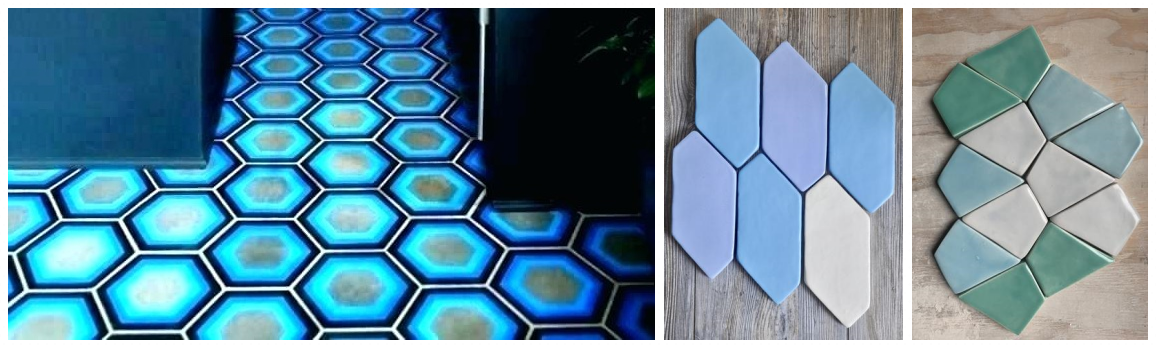
\includegraphics[width=330bp]{porcelana}
\caption{Ladrilhamentos usando polígonos de um só tipo. Fonte: Google imagens}
\label{porce}
\end{figure}

\vspace{-5mm}
\begin{task}{Ladrilhamentos usando triângulos}\label{at_lad_tri}

\textbf{Parte 1:} Copie a forma de um dos triângulos do encarte em um papel de gramatura mais alta. Recorte o triângulo. Crie um desenho, traçando repetidamente o triângulo. Verifique se a folha de papel está coberta e se não há espaços entre os triângulos.

\textbf{Parte 2:} Vamos explorar  ladrilhamentos  usando triângulos. 
\begin{enumerate}

\item Sugerimos que em um primeiro momento utilize o  \href{https://www.geogebra.org/m/uuafzw8k}{aplicativo}  para construir um ladrilhamento do plano usando apenas triângulos equiláteros. Para isso, procure distribuir os triângulos ao redor de um vértice.

\item Utilize o  \href{https://www.geogebra.org/m/junvq3qd}{aplicativo} e escolha um dos três triângulos para construir um novo ladrilhamento usando apenas triângulos.
\item Qual a diferença do primeiro ladrilhamento construído para o segundo?
\item Utilize o  \href{https://www.geogebra.org/m/ejfw44rt}{aplicativo}. Depois responda as questões:
\begin{enumerate}
\item O ladrilhamento que você produziu no item a pode ser reproduzido nesse aplicativo?
\item 	Peças triangulares de formato irregular podem ser usadas para ladrilhar o plano? O que torna um triângulo irregular?
\item  Se os ladrilhos triangulares são congruentes, eles podem ser usados para formar um ladrilhamento? Como você pode saber se triângulos  são congruentes ou não? Explique seu raciocínio.
\item 	Ao construir os seus ladrilhamentos (item a e b) a interseção entre dois polígonos era um um lado ou um vértice do triângulo? Isso é importante? Justifique! 
\item Escreva um breve parágrafo explicando quais informações geométricas você usou para criar seus ladrilhamentos? 
\end{enumerate}
\end{enumerate}

\end{task}

\begin{task}{Ladrilhamentos usando quadriláteros} \label{lad_qua}

\textbf{Parte 1:} Copie a forma de um quadrilátero do encarte em um papel de gramatura mais alta. Recorte-o. Crie um novo ladrilhamento usando o mesmo processo usado na Parte 1 da \hyperref[at_lad_tri]{atividade \ref{at_lad_tri}}. 

\textbf{Parte 2:} Vamos explorar  ladrilhamentos  usando quadriláteros. 
\begin{enumerate}

\item Utilize o \href{https://www.geogebra.org/m/d6nvffqk}{aplicativo} e escolha um dos quadriláteros para construir um ladrilhamento. Apenas observe que a interseção entre dois polígonos seja um lado ou um vértice.
\item Utilize o \href{https://www.geogebra.org/m/mdybnpnq}{aplicativo} e escolha um dos quadriláteros para construir um novo ladrilhamento.
\item Qual a diferença nos ladrilhamentos construídos nos itens a) e b) ?
\item Utilize o \href{https://www.geogebra.org/m/uqemfkhp#material/bhuqetbc}{aplicativo}. Depois responda as questões:
\begin{enumerate}
\item O ladrilhamento que você produziu nos itens a) e b) podem ser reproduzidos nesse aplicativo?
\item Os quadriláteros não convexos podem ser usados para criar ladrilhamentos interessantes. O que caracteriza um quadrilátero não convexo?
\end{enumerate}

\end{enumerate}

\end{task}


\begin{task}{Ladrilhamentos usando pentágonos}\label{lad_pen}

\textbf{Parte 1:} Copie a forma de  um pentágono do encarte em um papel de gramatura mais alta. Recorte-o. Crie um novo ladrilhamento usando o mesmo processo usado na Parte 1 da \hyperref[at_lad_tri]{atividade \ref{at_lad_tri}}. 

\textbf{Parte 2:} Vamos explorar  ladrilhamentos  usando pentágonos. 
\begin{enumerate}

\item Utilize o \href{https://www.geogebra.org/m/exzjd4mh}{aplicativo} para construir um ladrilhamento usando pentágonos regulares.
\item Utilize o  \href{https://www.geogebra.org/m/sffzzsww}{aplicativo}  e escolha um dos pentágonos para construir um novo ladrilhamento.
\item Qual a diferença nos ladrilhamentos construídos nos itens a) e b) ?
\end{enumerate}
\end{task}

\begin{task}{Ladrilhamentos usando hexágonos} \label{lad_hex}

\textbf{Parte 1:} Copie a forma de  um hexágono do encarte em um papel de gramatura mais alta. Recorte-o. Crie um novo ladrilhamento usando o mesmo processo usado na Parte 1 da \hyperref[at_lad_tri]{atividade \ref{at_lad_tri}}. 

\textbf{Parte 2:} Vamos explorar  ladrilhamentos  usando  hexágonos. 
\begin{enumerate}

\item Utilize o  \href{https://www.geogebra.org/m/uqemfkhp#material/zfczbshq}{aplicativo} para construir um ladrilhamento usando hexágonos regulares.
\item Utilize o  \href{https://www.geogebra.org/m/uqemfkhp#material/pnhc6tep}{aplicativo} e ladrilhe o plano com o hexágono disponível.
\item Qual a diferença nos ladrilhamentos construídos nos itens a) e b) ?

\item Utilize o \href{https://www.geogebra.org/m/uqemfkhp#material/ub84tqyy}{aplicativo} movimente os pontos azuis e responda: Quais propriedades o hexágono precisa ter para ladrilhar o plano?

\end{enumerate}
\end{task}




\begin{task}{Que formas podem ser usadas para ladrilhar o plano?}\label{at_formas}
\begin{enumerate}

\item Considere os polígonos da primeira coluna da tabela.  Meça cada ângulo interior e registre suas medidas na tabela.

\item Com base no que foi feito nos itens anteriores quais polígonos ladrilham o plano? Registre suas respostas na tabela.

% Não está aparecendo o cabeçalho no pdf 

\begin{table}[H]
\centering
\begin{tabular}{|l|c|c|}
\hline
\tcolor{\centering{Polígono}} & \tcolor{\makecell{Medida de \\ cada ângulo \\ interno}} & \tcolor{\makecell{Previsão: \\ O polígono \\ ladrilha o plano?}}  \\
\hline
Triângulo Equilátero & &  \\
\hline
Triângulo isóceles & &  \\
\hline
Quadrado & &  \\
\hline
Pentágono regular & &  \\
\hline
Hexágono regular & &  \\
\hline
Quadrilátero irregular & &  \\
\hline
Pentágono irregular & &  \\
\hline
Hexágono irregular & &  \\
\hline
\end{tabular}
\end{table}

\item Utilize o  \href{https://www.geogebra.org/m/uqemfkhp#material/eqwhddse}{aplicativo} para responder a seguinte questão:  Além dos polígonos citados na tabela, existem outros polígonos regulares  que ladrilham o plano?  Justifique!

\item Explique por que alguns polígonos ladrilham o plano, mas outros não. Existe um padrão?


\end{enumerate}

\end{task}

\arrange{Ladrilhando com polígonos do mesmo tipo}


Os ladrilhamentos com peças quadrangulares são comuns nos cômodos de nossas casas. As peças podem ser pintadas, esculpidas ou possuir saliências e combinadas formam as decorações dos ambientes, como ilustra a \hyperref[lad_qd]{figura \ref{lad_qd}}.
 


\begin{figure}[H]
\centering
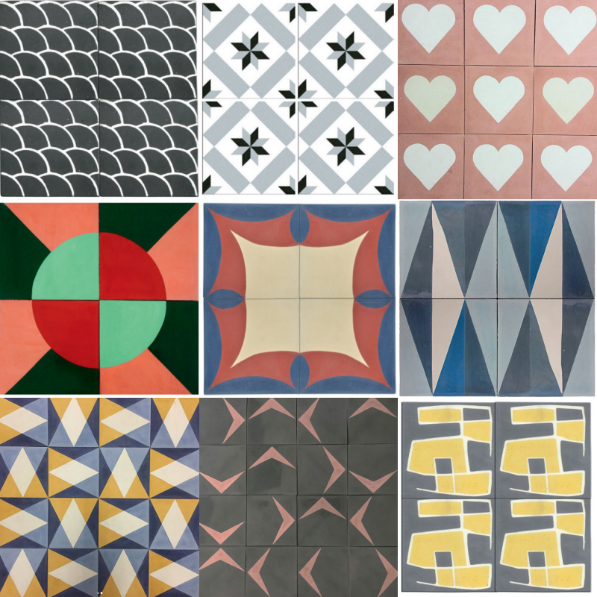
\includegraphics[width=180bp]{ladrilhamento14}
\caption{Peças quadrangulares. Fonte: Google Imagens }
\label{lad_qd}
\end{figure}

Também existem ladrilhamento hexagonais, apesar de menos usuais. Eles são encontrados em algumas pavimentações de ruas e áreas externas, nos favos, onde é armazenado o mel das abelhas. Também são comuns na confecção de colchas de retalhos  ou  de crochê (\hyperref[lad_hex]{figura \ref{lad_hex}}.

\begin{figure}[H]
\centering
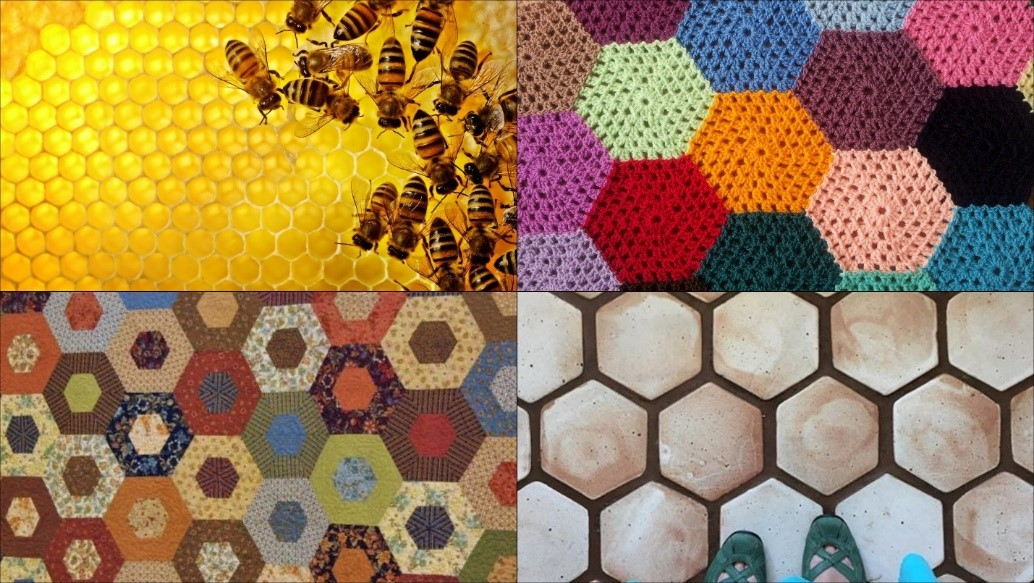
\includegraphics[width=250bp]{ladrilhamento15}
\caption{Peças hexagonais. Fonte: Google Imagens }
\label{lad_hex}
\end{figure}

Nas atividades anteriores, foram propostas tarefas utilizando vários tipos de polígonos, regulares e irregulares. Em todas as atividades, solicitamos que fosse utilizado apenas um tipo de polígono. Assim, foram construídos ladrilhamentos monoédricos. Os ladrilhamentos desse tipo são os constituídos de polígonos congruentes entre si. No caso, onde são usados polígonos regulares do mesmo tipo, os ladrilhamentos monoédricos são chamados de ladrilhamentos regulares.

Em cada uma das atividades anteriores procuramos colocar os polígonos (regulares e irregulares) de um determinado tipo ao redor de um vértice de forma que ficassem “lado a lado” (observando para que a interseção entre dois polígonos seja um lado ou um vértice). Isso significa que não consideramos ladrilhamentos como o ilustrado na \hyperref[ladr_tri1]{figura \ref{ladr_tri1}}. 

\begin{figure}[H]
\centering
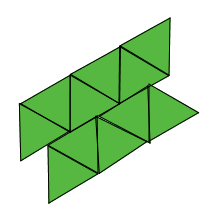
\includegraphics[width=150bp]{ladr_tri1}
\caption{Ladrilhamento com triângulos equiláteros.}
\label{ladr_tri1}
\end{figure}


Observamos que qo distribuir os polígonos ao redor do vértice,  temos duas possiblidades (\hyperref[lad_reg]{figura \ref{lad_reg}}): 
\begin{itemize}
\item	Completamos “a volta” e os polígonos se ajustam;
\item 	Não completamos a volta e se colocarmos mais um polígono, haverá uma sobreposição.
\end{itemize}


\begin{figure}[H]
\centering
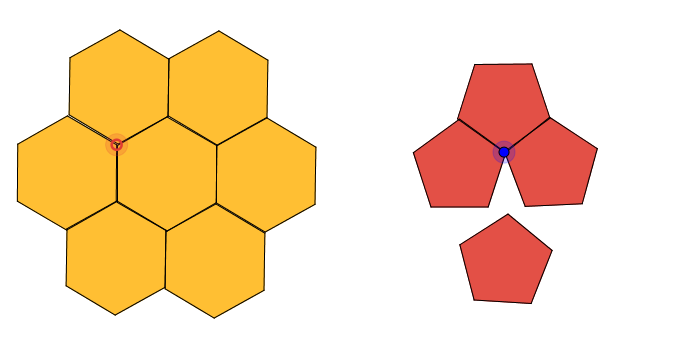
\includegraphics[width=300bp]{ladmon}
\caption{Disposição dos polígonos ao redor de um ponto.}
\label{lad_reg}
\end{figure}

Em um primeiro momento trabalhamos com triângulos equiláteros, e percebemos que é possível colocar perfeitamente seis triângulos equiláteros ao redor de um vértice e ao tomarmos um novo vértice, é possível continuar o ladrilhamento (\hyperref[ladr_tri2]{figura \ref{ladr_tri2}}). Ou seja,  os ladrilhamentos que vamos construir serão sempre pensados de forma a preencher todo um plano, ilimitado em todas as direções. 

\begin{figure}[H]
\centering
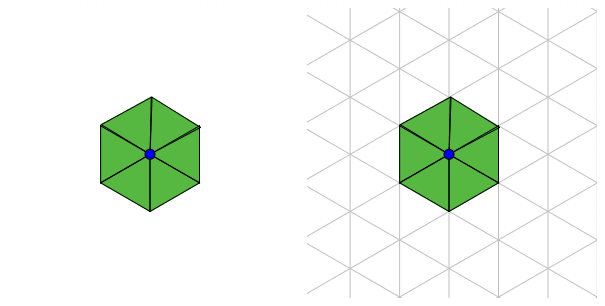
\includegraphics[width=300bp]{lad_tri2}
\caption{Triângulos ao redor de um vértice.}
\label{ladr_tri2}
\end{figure}
 
 
Na \hyperref[at_formas]{atividade \ref{at_formas}} solicitamos que os ângulos dos polígonos fossem medidos. Isso se justifica, pois, uma condição para que um polígono possa ladrilhar o plano é que a soma dos vários ângulos que se posicionam em torno de cada vértice resulte em um ângulo de $360 ^{\circ}$, como ilustra a \hyperref[angulos]{figura \ref{angulos}}.

\begin{figure}[H]
\centering
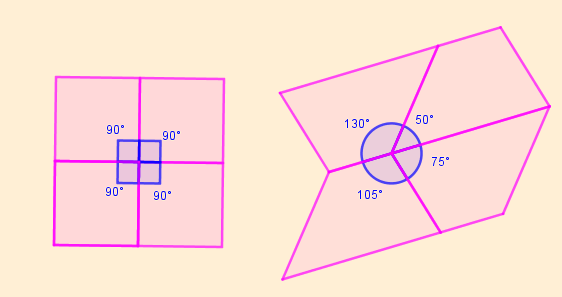
\includegraphics[width=250bp]{ladrilhamento8}
\caption{Ângulos ao redor de um vértice.}
\label{angulos}
\end{figure}


Uma pergunta que precisamos responder é:  quais polígonos regulares, de mesmo tipo pavimentam o plano?

Um fato conhecido é que a medida dos ângulos internos de um polígono regular de $n$ lados é $\displaystyle \frac{180^{\circ}(n-2)}{n}$. Assim, para que se tenha um ladrilhamento formado exclusivamente por polígonos regulares de $n$ lados é preciso que a medida do ângulo interno ($a_n$) seja um divisor de $360^{\circ}$, ou seja,

\begin{equation*}
\frac{180^{\circ}(n-2)}{n}=180^{\circ} \left(1 - \frac{2}{n}\right)=\frac{360^{\circ}}{m},
\end{equation*}
para algum número natural $m\geq1$.

Daí vem,

\begin{equation*}
1-\frac{2}{n}=\frac{2}{m}.
\end{equation*}

Logo,
\begin{equation*}
\frac{1}{n}+\frac{1}{m}=\frac{1}{2}.
\end{equation*}

Como $n$ é o número de lados de um polígono regular, é um número natural maior ou igual a três. E como $m$ também é um número natural, as únicas soluções inteiras e positivas, possíveis para a equação anterior são $n=3$ (com $m=6$), $n=4$ (com $m=4$) e $n=6$ (com $m=3$). Essas soluções resultam em exatamente três ladrilhamentos e consistem em distribuir ao redor de cada vértice ou $6$ triângulos equiláteros, ou $4$ quadrados ou $3$ hexágonos regulares. Ou seja, existem apenas três tipos de ladrilhamentos regulares, ilustrados na \hyperref[ladr_reg]{figura \ref{ladr_reg}}. O   \href{https://youtu.be/y__0a7TDbfs}{vídeo} poderá auxiliar na sua compreensão.


\begin{figure}[H]
\centering
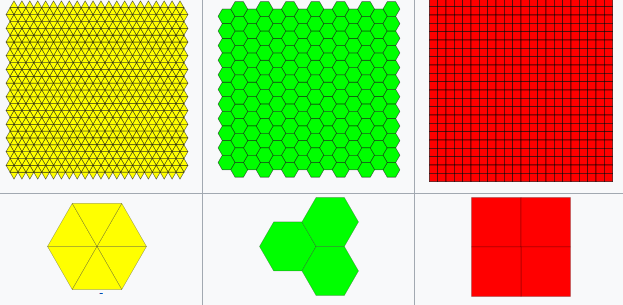
\includegraphics[width=400bp]{ladr_reg}
\caption{Ladrilhamentos regulares. Fonte \href{https://en.wikipedia.org/wiki/Euclidean_tilings_by_convex_regular_polygons}{Wikipedia}}
\label{ladr_reg}
\end{figure}



E quais polígonos irregulares de mesmo tipo ladrilham o plano?
 
Na \hyperref[lad_qua]{atividade \ref{lad_qua}} foi possível construir ladrilhamentos utilizando alguns quadriláteros, em particular com paralelogramos, que são quadriláteros que possuem os lados opostos paralelos. Afirmamos que os paralelogramos ladrilham o plano, pois possuem ângulos dois a dois suplementares e lados opostos congruentes (\hyperref[par]{figura \ref{par}}).

\begin{figure}[H]
\centering
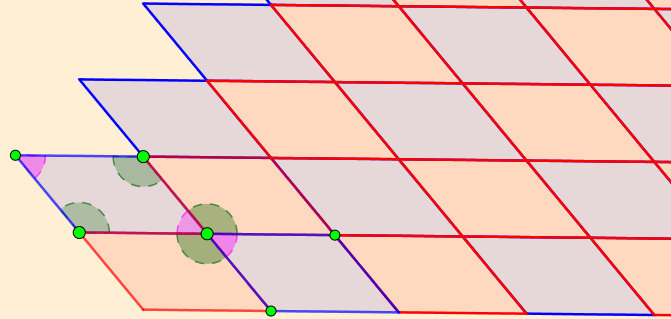
\includegraphics[width=350bp]{par}
\caption{Ladrilhamento com paralelogramos}
\label{par}
\end{figure}


Como os quadrados, losangos e retângulos são paralelogramos, eles também ladrilham o plano.
Porém, se consideramos um quadrilátero qualquer como proposto no item b) da mesma atividade, usamos quadriláteros quaisquer para ladrilhar o plano e no aplicativo disponível no item c) foi possível perceber que qualquer quadrilátero pode ladrilhar o plano. Como a  soma dos ângulos internos de qualquer quadrilátero é $360^{\circ}$, para construir um ladrilhamento usando quadriláteros, basta arranja-los ao redor do vértice, utilizando transformações isométricas, de forma a coincidir os lados. 

Na \hyperref[at_lad_tri]{atividade \ref{at_lad_tri}} usamos triângulos para compor ladrilhamentos. Observe que ao considerar um triângulo qualquer, como o da \hyperref[triqqr]{figura \ref{triqqr}} e traçar por dois vértices retas paralelas, respectivamente, aos outros lados, obtemos um paralelogramo. 

\begin{figure}[H]
\centering
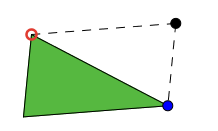
\includegraphics[width=200bp]{triqqr}
\caption{Triângulos.}
\label{triqqr}
\end{figure}

Consequentemente, seja qual for o triângulo, ele ladrilhará o plano.

Também tentamos utilizar pentágonos para ladrilhar o plano (na \hyperref[lad_pen]{atividade \ref{lad_pen}}). Nesse caso, percebemos que os pentágonos regulares não ladrilham o plano. Porém, no item b)da mesma atividade, foi possível verificar  que alguns pentágonos o fazem. Mas que tipo de pentágonos irregulares ladrilham o plano?

Em 2015 matemáticos da  Universidade de Washington Bothell, descobriram um pentágono irregular que ladrilha o plano. Antes desta descoberta, havia apenas quatorze tipos conhecidos de pentágonos irregulares capazes de ladrilhar o  plano, cuja descoberta varia do início ao final do século XX. Em 2017, com o auxílio de algoritmos computacionais, foi provado que são exatamente 15 tipos de pentágonos irregulares que ladrilham o plano (\hyperref[pentagono]{figura \ref{pentagono}}).

\begin{figure}[H]
\centering
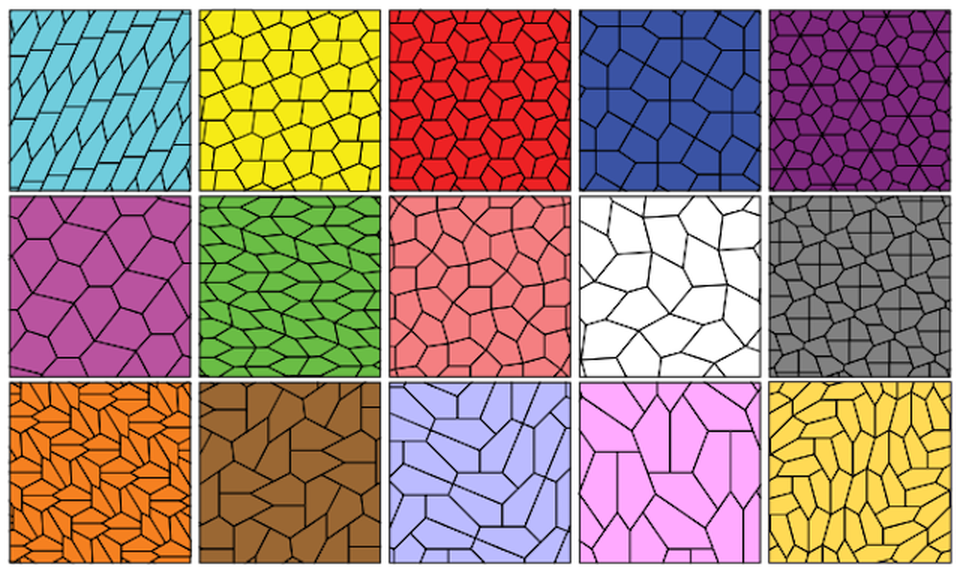
\includegraphics[width=400bp]{pentagono}
\caption{Ladrilhamentos com pentágonos irregulares. \href{encurtador.com.br/dmuE3}{Forbes}}
\label{pentagono}
\end{figure}



Na \hyperref[lad_hex]{atividade \ref{lad_hex}} produzimos ladrilhamentos usando hexágonos irregulares (itens b e d). No início do século XX, K. Reinhardt um matemático alemão provou que existem três tipos de hexágonos irregulares que pavimentam o plano. No que segue mostraremos como são esses tipos de hexágonos. Assim, vamos considerar um hexágono $ABCDEF$ irregular com lados de medidas $a$, $b$, $c$, $d$, $e$ e $f$ e ângulos de medidas $\hat{A}... \hat{F}$ como indicados na \hyperref[hex1]{figura \ref{hex1}}.

\begin{figure}[H]
\centering
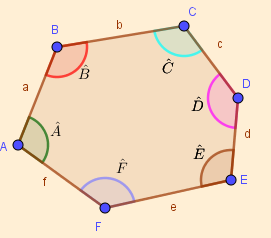
\includegraphics[width=200bp]{hex1}
\caption{Hexágono}
\label{hex1}
\end{figure}

O primeiro tipo de hexágono regular capaz de ladrilhar o plano, são aqueles que possuem um par de lados congruentes e paralelos. Consideremos, sem perda de generalidade, os lados $c$ e $f$ satisfazendo essas condições.  (\hyperref[hex2]{figura \ref{hex2}}.

\begin{figure}[H]
\centering
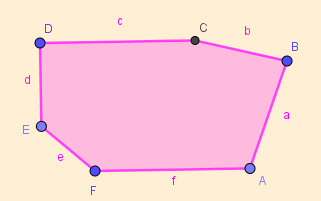
\includegraphics[width=200bp]{hex2}
\caption{Hexágono com um par de lados paralelos e congruentes.}
\label{hex2}
\end{figure}

 
Para realizar o ladrilhamento, vamos arranjar os polígonos no vértice $A$, por exemplo, de forma que os lados $c$ e $f$ coincidam e que o ângulo $\hat{B}$ coincida com $\hat{A}$ (\hyperref[hex3]{figura \ref{hex3}}).

\begin{figure}[H]
\centering
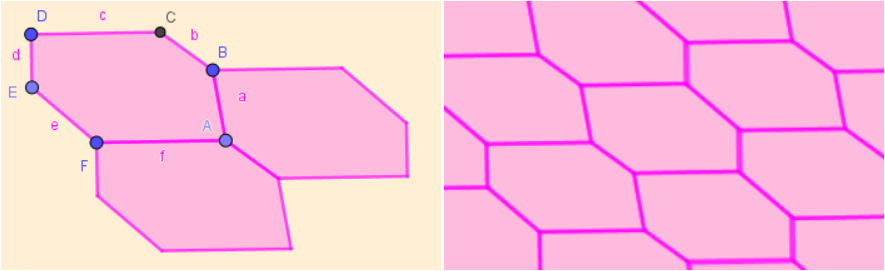
\includegraphics[width=400bp]{hex3}
\caption{Ladrilhamento com hexágonos do tipo 1.}
\label{hex3}
\end{figure}

Um fato importante de ser observado é que a condição um par de lados paralelos ($AF//DC$ ou $f//c$)  é equivalente a $\hat{D} + \hat{E} + \hat{F} = 360^{\circ}$.

De fato,  considerando que o segmento $AC$ divide o ângulo $\hat{A}$ em outros dois ângulos $\alpha$ e $\beta$ e o ângulo $\hat{C}$ nos ângulos $\delta$ e $\gamma$ (\hyperref[hex4]{figura \ref{hex4}}).


\begin{figure}[H]
\centering
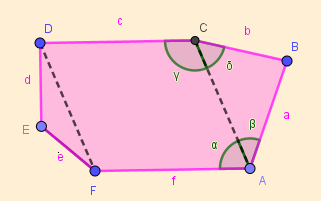
\includegraphics[width=200bp]{hex4}
\caption{Ângulos no hexágono.}
\label{hex4}
\end{figure}

E, como os lados $AF$ e $DC$ são paralelos, segue que $\alpha +\gamma = 180^{\circ}$.

Mas, $$\hat{A} + \hat{B} + \hat{C} = \alpha + \beta + \hat{B} + \gamma + \delta.$$

Logo, $\hat{A} + \hat{B} + \hat{C} = 360^{\circ}$. Pois  $\beta + \hat{B} + \gamma = 180^{\circ}$ (ângulos internos do triângulo ABC).

Reciprocamente, supondo que $\hat{A} + \hat{B} + \hat{C} = 360^{\circ}$ resulta que  $\alpha +\gamma = 180^{\circ}$ ou que $AF//DC$.

Como a soma dos ângulos internos de um hexágono é $720^{\circ}$ resulta que a condição $AF//DC$ também equivale a $\hat{D} + \hat{E} + \hat{F} = 360^{\circ}$.



Os hexágonos classificados como  como do segundo tipo são o que satisfazem as seguintes condições: $c= f$, $b=d$ e  $\hat{A} + \hat{B} + \hat{D} = 360^{\circ}$ (figura \ref{hex5}).

\begin{figure}[H]
\centering
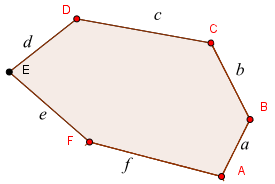
\includegraphics[width=200bp]{hex5}
\caption{Hexágonos do tipo 2.}
\label{hex5}
\end{figure}


Para realizar o ladrilhamento com esse tipo de polígono, os hexágonos devem ser arranjados em torno de um vértice ($A$, por exemplo)  de modo que o lado de medida $c$ coincida com o lado de medida $f$ e o lado de medida $b$ coincida com o lado de medida $d$ (\hyperref[hex6]{figura \ref{hex6}}).

\begin{figure}[H]
\centering
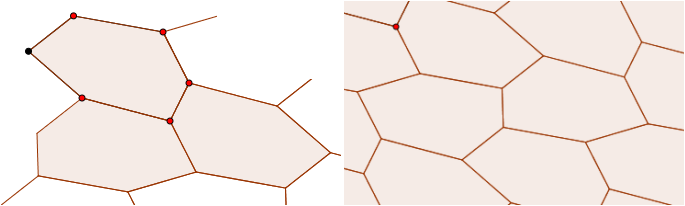
\includegraphics[width=400bp]{hex6}
\caption{Ladrilhamento com hexágonos do tipo 2.}
\label{hex6}
\end{figure}

No item d) da \hyperref[lad_hex]{atividade \ref{lad_hex}} apresentamos o terceiro tipo de hexágonos que ladrilham o plano. Nesse tipo, os lados adjacentes são congruentes e os ângulos entre esses lados são congruentes e medem $120^{\circ}$. Na \hyperref[hex7]{figura \ref{hex7}}, $a=f$, $b=c$, $d=e$ e $\hat{A}=\hat{C}=\hat{E}= 120^{\circ}$.

\clearmargin

\def\currentcolor{session2}
\begin{objectives}{Ladrilhando com losangos}
{
	Reconhecer que os losangos  ladrilham o plano.	
}{1}{0}
\end{objectives}
\begin{sugestions}{Ladrilhando com losangos}
{
	Estas atividades, foram pensadas para serem realizadas com o uso de ferramentas computacionais. Pretende-se com o uso dessas ferramentas chamar a atenção para os diferentes tipos de ladrilhamentos e realizar comparações entre eles e reconhecer qual a razão para os ladrilhamentos serem possíveis. 

	\textbf{Organização em sala de aula}: Recomenda-se que os estudantes trabalhem em duplas, de preferência em um laboratório de informática, onde o aplicativo GeoGebra esteja previamente instalado.
}{1}{0}
\end{sugestions}
\begin{answer}{Ladrilhando usando losangos}
{
	\begin{enumerate}
	\item É um losango que possui os ângulos de de $60^{\circ}$ e $120^{\circ}$
	\item Sim, como os ângulos são dois a dois suplementares, em todo o nó se tem $360^{\circ}$.Um outro ladrilhamento possível é o ilustrado na figura:
	\begin{figure}[H]
	\centering
	
	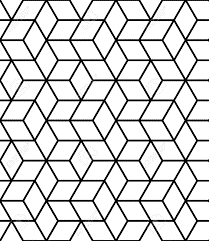
\includegraphics[width=125bp]{ladrilhamento-professor23}
	\end{figure}
	\end{enumerate}
}{1}
\end{answer}
\clearmargin
\begin{objectives}{Ladrilhamentos usando trapézios}
{
	\begin{itemize}
	\item Analisar os tipos de ladrilhamentos que podem ser construídos usando trapézios.
	\end{itemize}
}{1}{1}
\end{objectives}
\begin{sugestions}{Ladrilhamentos usando trapézios}
{
	Estas atividades, foram pensadas para serem realizadas com o uso de lápis e papel. Pretende-se com a atividade chamar a atenção para os diferentes tipos de ladrilhamentos e criados comparando entre eles e reconhecer quais padrões encontrado. 

	\textbf{Organização em sala de aula}: Recomenda-se que os estudantes trabalhem individualmente. E no final seja realizado um compartilhamento dos diferentes resultados.
}{1}{1}
\end{sugestions}
\begin{answer}{Ladrilhamentos usando trapézios}
{
	\begin{enumerate}
	\item Um trapézio é um quadrilátero, e como a soma dos ângulos internos de qualquer quadrilátero é $360^{\circ}$, ele ladrilha o plano.
	\item
	\begin{enumerate}
	\item 
	\adjustbox{valign=t}
	{
	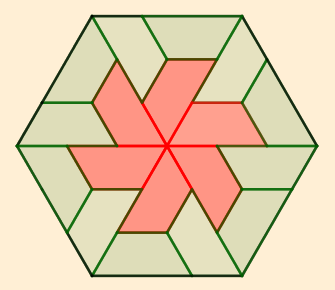
\includegraphics[width=150bp]{ladrilhamento-professor24}
	}

	\item
	\adjustbox{valign=t}
	{	
	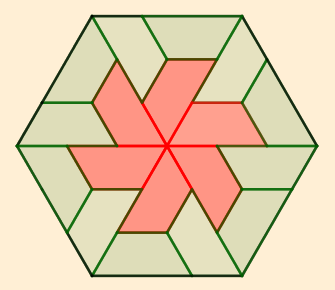
\includegraphics[width=150bp]{ladrilhamento-professor24}
	}
	\end{enumerate}
	\end{enumerate}
}{1}
\end{answer}

\clearmargin
\begin{objectives}{Ladrilhamento dual}
{
	\begin{itemize}
	\item Analisar os tipos de ladrilhamentos presentes e reconhecê-los.
	\item Criar novas suposições, seguindo o raciocínio exposto
	\end{itemize}
}{1}{1}
\end{objectives}
\begin{sugestions}{Ladrilhamento dual}
{
	Estas atividades, foram pensadas para serem realizadas com o uso de lápis e papel. Pretende-se com a atividade chamar a atenção para uma maneira diferente de criar  ladrilhamentos, utilizando os ladrilhamentos já conhecidos, além de  reconhecer quais padrões são encontrados. 

	\textbf{Organização em sala de aula}: Recomenda-se que os estudantes trabalhem individualmente ou em duplas.
}{1}{1}
\end{sugestions}
\begin{answer}{Ladrilhamento dual}
{
	\begin{figure}[H]
	\centering
	
	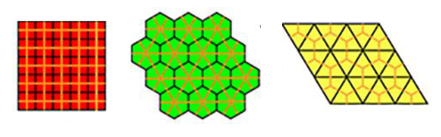
\includegraphics[width=.8\linewidth]{reviso4}
	\end{figure}
}{1}
\end{answer}

\begin{figure}[H]
\centering
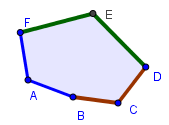
\includegraphics[width=200bp]{hex7}
\caption{Hexágonos do tipo 3.}
\label{hex7}
\end{figure}

Para construir um ladrilhamento com esse tipo de polígono, basta arranjar os hexágono de forma que os ângulos de $120^{\circ}$ estejam posicionados em torno de um vértice (\hyperref[hex8]{figura \ref{hex8}}), observando para que os lados congruentes coincidam.

\begin{figure}[H]
\centering
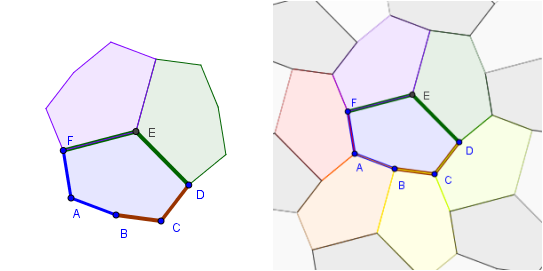
\includegraphics[width=300bp]{hex8}
\caption{Ladrilhamento com hexágonos do tipo 3.}
\label{hex8}
\end{figure}


Quanto aos demais polígonos irregulares convexos (com mais de 7 lados) esses não ladrilham o plano, pois não é possível realizar um arranjo desse tipo de polígono em torno de um vértice, sem que tenhamos espaços em branco ou sobreposições.

Observamos que nesse primeiro momento trabalhamos com ladrilhamentos monoédricos, ou seja, formados por ladrilhos de um só tipo. Mas se  ladrilhos forem polígonos regulares, de vários tipos. O que ocorre?



\practice{Vamos ladrilhar}


\begin{task}{Ladrilhamentos usando losangos}

Um losango (que também é um paralelogramo) fornece um padrão que cria a aparência de cubos em perspectiva, como ilustra a \hyperref[losango]{figura \ref{losango}}.

	\begin{figure}[H]
	\centering
	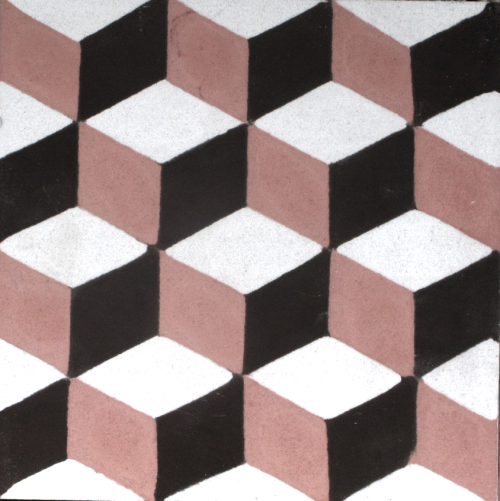
\includegraphics[width=150bp]{ladrilhamento47}
    \caption{Ladrilhamento com losangos}
   	\label{losango}
	\end{figure}
	
\begin{enumerate}
			\item O que esse losango possui de especial?
			\item Será que é possível construir outro tipo de ladrilhamento com esses losangos? (Use o GeoGebra ou os losangos do encarte)
\end{enumerate}
\end{task}

\begin{task}{Ladrilhamentos usando trapézios}
\begin{enumerate}
\item Será que é possível ladrilhar o plano usando trapézios? Justifique.

\item Um trapézio muito interessante, chamado 60-120 (\hyperref[trap1]{figura \ref{trap1}}, quando se trata de ladrilhamento, é o constituído por três triângulos equiláteros.

\begin{figure}[H]
\centering
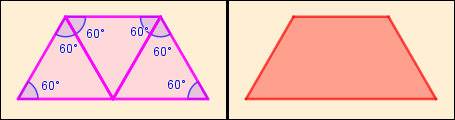
\includegraphics[width=300bp]{ladrilhamento48}
\caption{Trapézio.}
\label{trap1}
\end{figure}

\begin{enumerate}
	\item A \hyperref[trap2]{figura \ref{trap2}} ilustra um ladrilhamento parcial feito com esse trapézio, em um hexágono regular (e como o hexágono ladrilha o plano, basta repetir o padrão hexagonal). Construa outro ladrilhamento parcial no hexágono usando apenas trapézios 60-120.

	\begin{figure}[H]
	\centering
	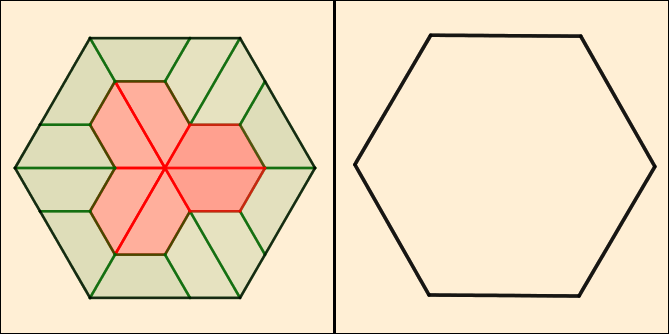
\includegraphics[width=250bp]{ladrilhamento49}
	\caption{Ladrilhamento parcial}
	\label{trap2}
	\end{figure}

	\item Com o trapézio 60-120 também é possível construir ladrilhamentos do tipo faixas decorativas, como ilustra a \hyperref[trap3]{figura \ref{trap3}}. 

	\begin{figure}[H]
	\centering
	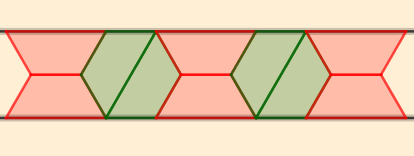
\includegraphics[width=300bp]{ladrilhamento50}
	\caption{Faixa decorativa}
     \label{trap3}
	\end{figure}
	
Faça um ladrilhamento diferente do apresentado usando trapézios 60-120.

\end{enumerate}
\end{enumerate}
\end{task}


\clearpage

\begin{task}{Ladrilhamento dual}
O diagrama a seguir ilustra um ladrilhamento de quadrados. Adicionando um ponto ao centro de cada quadrado e unindo-os formando quadrados adjacentes, formamos um novo ladrilhamento, que se denomina dual do ladrilhamento original.

	\begin{figure}[H]
	\centering
	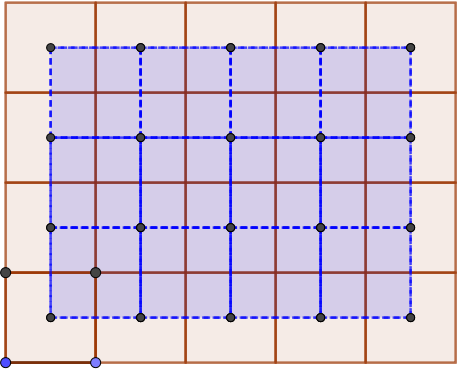
\includegraphics[width=250bp]{dual}
	\caption{Ladrilhamento Dual}
	\end{figure}

	\begin{enumerate}
		\item Que tipo de ladrilhamento é o dual do ladrilhamento de quadrados original?
		\item Desenhe um ladrilhamento de hexágonos regulares. Desenhe e descreva o seu dual;
		\item Desenhe um ladrilhamento de triângulos equiláteros. Desenhe e descreva o seu dual.
	\end{enumerate}

\end{task}



%%%%%%%%%%%%%%%%%%%%%%%%

\cleardoublepage
\def\currentcolor{session1}
\begin{objectives}{Ladrilhando o plano com polígonos de mais de um tipo}
{
	\begin{itemize}
	\item Reconhecer que é possível ladrilhar o plano com dois ou mais polígonos regulares
	\item \textbf{Conceitos abordados}: Ladrilhamentos semirregulares
	\end{itemize}
}{1}{1}
\end{objectives}
\begin{sugestions}{Ladrilhando o plano com polígonos de mais de um tipo}
{
Tenha  em mente alguns exemplos de ladrilhamenos semirregulares, incentivando os alunos a terems êxito na  atividade.

Relembrar os ângulos internos de cada polígono regular pode ser útil. Deixando uma dica aos alunos para pensar nisso antes de escolher seus polígonos.

\textbf{Organização em sala de aula}:Para realizar essa atividade, deve-se distribuir aos alunos ( ou grupos) polígonos regulares de tipos diferentes. Nesta atividade, o aluno deverá construir ladrilhamentos com polígonos regulares de tipos diferentes. O ideal é que ele faça isso em grupos de no máximo 4 alunos, para que possam discutir sobre as construções realizadas. 

\textbf{Dificuldades previstas}: É possível que inicialmente os alunos tenham alguma dificuldade, principalmente devido ao desafio proposto. Observa-se que a descoberta via experimento utilizando polígonos regulares de diferentes tipos congruentes entre si, pode ser realizada, como foi feito para polígonos regulares de um único tipo. Porém, é preciso ter cuidado, pois poderá conduzir a conclusões errôneas, se não for observado a soma dos ângulos internos dos polígonos que circundam um vértice, no sentido de verificar se essa soma é, ou não, igual a 360º. Os enganos podem ocorrer visto pequenas imperfeições no material utilizado, ou por erros de aproximação do tipo visual. No exemplo (figura) tem-se um pentágono, um hexágono e um octógono regulares. Nesse caso, a soma dos ângulos é 363º, o que ultrapassa em apenas 3º o valor de uma volta completa.

\begin{figure}[H]
\centering

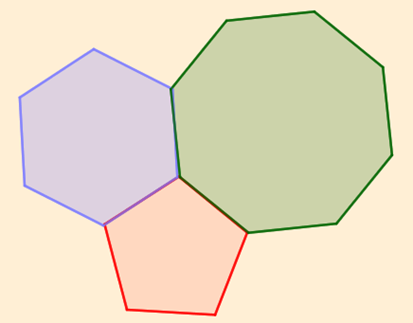
\includegraphics[width=150bp]{reviso5}
\end{figure}

}{1}{1}
\end{sugestions}
\begin{sugestions}{Ladrilhando o plano com polígonos de mais de um tipo}
{
	\textbf{Sugestões gerais}: Espera-se que os alunos consigam chegar à conclusão que existem exatamente 8 tipos de mosaicos semirregulares sendo obtidos com 2 ou, no máximo, 3 tipos de polígonos regulares. Observa-se que nem todos os polígonos regulares podem ser usados para fazer ladrilhamentos semirregulares. Por exemplo, pentágonos, heptágonos, eneágonos e decágonos regulares não compõem ladrilhamentos semirregulares, mas é importante que os alunos tentem fazer ladrilhamentos usando esses tipos de polígonos. 
	Para o desenvolvimento da tarefa, recomenda-se ainda que o professor prepare o material com antecedência, imprimindo os polígonos do encarte em papel cartão, ou solicitando que os alunos o façam. Caso opte por utilizar material digital, indicamos o site http://www.cdme.im-uff.mat.br/ppr/ppr-html/ppr-st-br.html . Apenas verifique com antecedência se o mesmo está funcionando de forma satisfatória. 
	 
	\textbf{Enriquecimento da discussão}: Sugere-se ainda que o professor incentive seus alunos a perceber quais as combinações produzem ladrilhamentos e quais os padrões que estão sendo formados.

	\textbf{Material necessário}: Polígonos impressos do encarte em folha de gramatura mais alta ou impressos em 3D	
}{0}{1}
\end{sugestions}

\explore{Ladrilhando com polígonos regulares}



\begin{task}{Ladrilhando o plano com polígonos de mais de um tipo}\label{ladtipos}

\textbf{Parte 1 :} Escolha dois polígonos regulares diferentes que possam ser usados para criar um ladrilhamento. 
\begin{enumerate}
\item Quais polígonos regulares foram escolhidos?
\item Desenhe o ladrilhamento usando papel milimetrado usando os dois polígonos regulares. 
\item É possível fazer um ladrilhamento, arranjando  apenas dois polígonos regulares ao redor de um vértice? Justifique! 
\end{enumerate}

\textbf{Parte 2:} Escolha três polígonos regulares diferentes que possam ser usados para criar um ladrilhamento. 
\begin{enumerate}
\item Quais polígonos regulares foram escolhidos?
\item Desenhe o ladrilhamento usando papel milimetrado usando os dois polígonos regulares. 
\item É possível fazer um ladrilhamento, arranjando  apenas três polígonos regulares ao redor de um vértice? Justifique! 
\end{enumerate}


\textbf{Parte 3:} Repita o procedimento realizado na \textbf{Parte 2 }usando 4,5, 6 e 7 polígonos regulares.

\textbf{Parte 4:} Socialize suas respostas com os colegas.

\end{task}


\arrange{Ladrilhando com polígonos regulares}

Na \hyperref[ladtipos]{atividade \ref{ladtipos}} investigamos  quais os tipos de ladrilhamentos, cujos ladrilhos são polígonos regulares de mais de um tipo, podem ser construídos. Esses ladrilhamentos são denominados semirregulares. Alguns desses ladrilhamentos são encontrados em revestimentos de pisos. Alguns são formados por quadrados e octógonos regulares  e outros são formados por quadrados, triângulos equiláteros e hexágonos regulares (\hyperref[lad_tp1]{figura \ref{lad_tp1}}).


\begin{figure}[H]
\centering
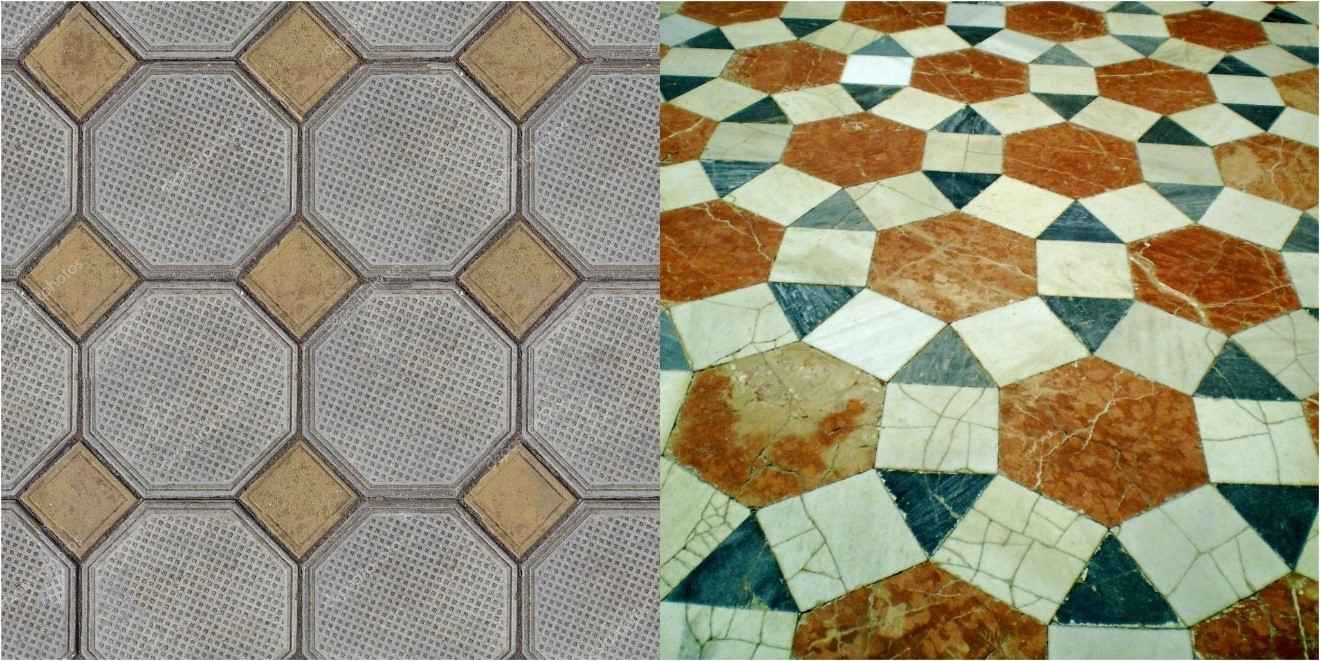
\includegraphics[width=300bp]{ladrilhamento18}
\caption{Revestimentos. Fonte: Google Imagens}
\label{lad_tp1}
\end{figure}

Um arranjo de polígonos regulares ao redor de um determinado vértice é denominado de configuração. E existe uma notação para ela, que se deve ao número de lados dos polígonos regulares que constituem o arranjo. Por exemplo, a configuração 4-8-8 significa que ao redor de um vértice há um quadrado,  um octágono regular e um octágono regular, nesta ordem e em qualquer vértice do ladrilhamento. Já a configuração 3- 4- 6- 4 significa que ao redor de um vértice há um triângulo equilátero, um quadrado, um hexágono regular e um quadrado, nesta ordem e em qualquer vértice do ladrilhamento (\hyperref[lad_tp2]{figura \ref{lad_tp2}}).


\begin{figure}[H]
\centering
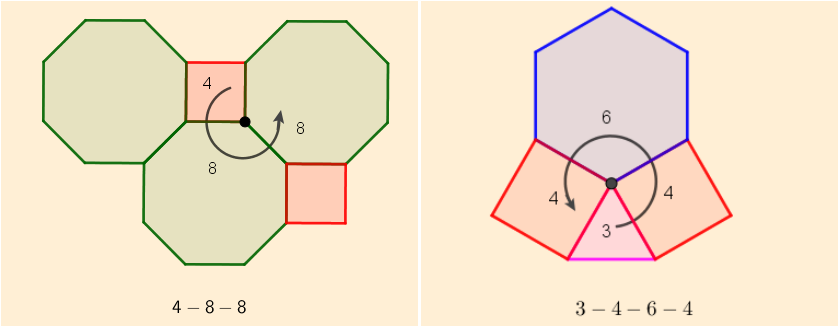
\includegraphics[width=350bp]{ladtp_2}
\caption{Configuração.}
\label{lad_tp2}
\end{figure}

A existência de ladrilhamentos  cujas peças são polígonos regulares já era conhecida pelos antigos pitagóricos da Matemática grega. Porém, a primeira pessoa a exibir os ladrilhamentos regulares e semirregulares (formados por polígonos regulares de tipos diferentes) foi J. Kepler em um trabalho publicado no início do século XVII, onde consta o seguinte resultado:

\begin{observation}{Teorema de Kepler}
Existem exatamente 11 maneiras de se cobrir o plano utilizando-se exclusivamente polígonos regulares sujeitos as seguintes condições:
\begin{itemize}
\item	se dois polígonos regulares intersectam-se, então essa interseção é um lado ou um vértice comum.
\item	A distribuição dos polígonos regulares ao redor de cada vértice é sempre a mesma.
\end{itemize}

\end{observation}



\begin{knowledge}
Johannes Kepler (1571-1630), em sua obra \textit{Harmonia do Mundo}, de 1619,trouxe as primeiras investigações referentes à teoria da pavimentação do plano euclidiano utilizando polígonos regulares, apontando um tratamento matemático para o problema.
\end{knowledge}




Assim, considerando que em torno de um vértice podemos colocar um número $k$ de polígonos regulares, e que $60^{\circ}$ é o menor ângulo interno de um polígono regular, então o maior valor de $k$ é dado por $\displaystyle \frac{360^{\circ}}{60^{\circ}} = 6$, que corresponde a 6 triângulos equiláteros. Por outro lado, o menor número de polígonos regulares  necessários para realizar um ladrilhamento em torno de um vértice é 3, temos  $3\leq k \leq 6$.

Observa-se então que será possível construir ladrilhamentos do plano com 3, 4, 5 ou 6 polígonos regulares em torno de cada vértice (\hyperref[lad_tp3]{figura \ref{lad_tp3}}).

\begin{figure}[H]
\centering
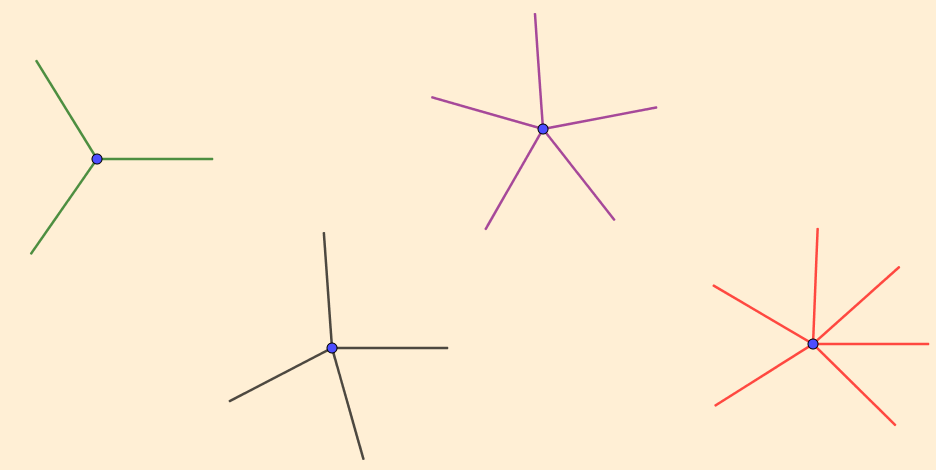
\includegraphics[width=300bp]{ladrilhamento21}
\caption{Número de polígonos em torno de um vértice.}
\label{lad_tp3}
\end{figure}

Examinaremos cada um dos casos separadamente.

Considerando $k=3$, ou seja, supondo que três polígonos regulares são arranjados em torno de um vértice de modo que não haja nem lacunas nem sobreposições, o primeiro com $n_1$ lados, o segundo com $n_2$ lados e o terceiro com $n_3$ lados (\hyperref[lad_tp4]{figura \ref{lad_tp4}}).

\begin{figure}[H]
\centering
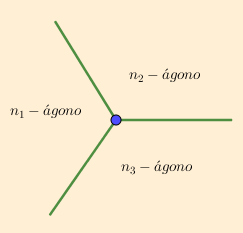
\includegraphics[width=200bp]{ladrilhamento22}
\caption{Número de polígonos regulares em torno de um vértice.}
\label{lad_tp4}
\end{figure}

Como o ângulo interno de cada $n_i$-ágono, com $i=1,2,3$ é dado por

\begin{equation*}
180^{\circ}\left(1-\frac{2}{n_i}\right)
\end{equation*}

E como a soma dos ângulos em torno de um vértice é $360^{\circ}$, temos

\begin{equation*}
180^{\circ}\left(1-\frac{2}{n_1}\right)+180^{\circ}\left(1-\frac{2}{n_2}\right)+180^{\circ}\left(1-\frac{2}{n_3}\right)=360^{\circ}.
\end{equation*}

Daí,

\begin{equation*}
\frac{1}{n_1}+\frac{1}{n_2}+\frac{1}{n_3}=\frac{1}{2}
\end{equation*}

Para determinar as soluções inteiras e positivas da equação anterior, vamos supor, sem perda de generalidade, que $n_1\leq n_2\leq n_3$.

Logo,

\begin{equation*}
\frac{1}{n_2}\leq\frac{1}{n_1},\quad \frac{1}{n_3}\leq\frac{1}{n_1},
\end{equation*}

e portanto,

\begin{equation*}
\frac{1}{2}=\frac{1}{n_1}+\frac{1}{n_2}+\frac{1}{n_3}\leq\frac{1}{n_1}+\frac{1}{n_1}+\frac{1}{n_1}=\frac{3}{n_1},
\end{equation*}

ou seja, $n_1\leq6$.

Suponhamos que $n_1=3$, ou seja, que um dos polígonos regulares dispostos ao redor do vértice seja um triângulo equilátero. Então,

\begin{equation*}
\frac{1}{3}+\frac{1}{n_2}+\frac{1}{n_3}=\frac{1}{2}.
\end{equation*}

Daí,

\begin{equation*}
\frac{1}{n_2}+\frac{1}{n_3}=\frac{1}{6}.
\end{equation*}

Ou ainda,

\begin{equation*}
\frac{1}{n_3}=\frac{n_2-6}{6n_2},
\end{equation*}

logo, $n_2\geq7$.

Por outro lado, como $n_2\geq n_3$, temos,

\begin{equation*}
\frac{n_2-6}{6n_2}=\frac{1}{n_3}\leq\frac{1}{n_2},
\end{equation*}

O que implica $n_2\leq12$.

Assim, substituindo os valores possíveis para $n_2$ e como $n_3$ é um número inteiro, obtemos as seguintes soluções:


\begin{table}[H]
\centering
\setlength\tabcolsep{5mm}
\begin{tabular}{|c|c|c|}
\hline
\tcolor{$\bm{n_1}$} & \tcolor{$\bm{n_2}$} & \tcolor{$\bm{n_3}$} \\
\hline
$3$ & $7$ & $42$ \\
\hline
$3$ & $8$ & $24$ \\
\hline
$3$ & $9$ & $18$ \\
\hline
$3$ & $10$ & $15$ \\
\hline
$3$ & $12$ & $12$ \\
\hline
\end{tabular}
\end{table}

Suponhamos agora que $n_1=4$, ou seja, que um dos polígonos regulares dispostos ao redor do vértice seja um quadrado. Então,

\begin{equation*}
\frac{1}{4}+\frac{1}{n_2}+\frac{1}{n_3}=\frac{1}{2}.
\end{equation*}

Daí,

\begin{equation*}
\frac{1}{n_2}+\frac{1}{n_3}=\frac{1}{4}.
\end{equation*}

Ou ainda,

\begin{equation*}
\frac{1}{n_3}=\frac{n_2-4}{4n_2},
\end{equation*}

logo, $n_2\geq5$.

Por outro lado, como $n_2\geq n_3$, temos,

\begin{equation*}
\frac{n_2-4}{4n_2}=\frac{1}{n_3}\leq\frac{1}{n_2},
\end{equation*}

o que implica $n_2\leq8$.

Assim, substituindo os valores possíveis para $n_2$ e como $n_3$ é um número inteiro, obtemos as seguintes soluções:


\begin{table}[H]
\centering
\setlength\tabcolsep{5mm}
\begin{tabular}{|c|c|c|}
\hline
\tcolor{${n_1}$} & \tcolor{${n_2}$} & \tcolor{${n_3}$} \\
\hline
$4$ & $5$ & $20$ \\
\hline
$4$ & $6$ & $12$ \\
\hline
$4$ & $8$ & $8$ \\ 
\hline
\end{tabular}
\end{table}

Procedendo de forma análoga, considerando $n_1 = 5$, temos $5\leq n_2 \leq6$ e uma única solução da equação

\begin{equation*}
\frac{1}{5}+\frac{1}{n_2}+\frac{1}{n_3}=\frac{1}{2}
\end{equation*}

é $n_2=5$ e $n_3=10$. E, considerando $n_1=6$, a única solução é $n_2 = 6$ e $n_3=6$.

Portanto, as soluções inteiras positivas da equação

\begin{equation*}
\frac{1}{n_1}+\frac{1}{n_2}+\frac{1}{n_3}=\frac{1}{2},
\end{equation*} 

estão descritas na tabela a seguir:

\begin{table}[H]
\setlength\tabcolsep{5mm}
\centering
\begin{tabular}{|c|c|c|}
\hline
\tcolor{$\bm{n_1}$} & \tcolor{$\bm{n_2}$} & \tcolor{$\bm{n_3}$} \\
\hline
$3$ & $7$ & $42$ \\
\hline
$3$ & $8$ & $24$ \\
\hline
$3$ & $9$ & $18$ \\
\hline
$3$ & $10$ & $15$ \\
\hline
$3$ & $12$ & $12$ \\
\hline
$4$ & $5$ & $20$ \\
\hline
$4$ & $6$ & $12$ \\
\hline
$4$ & $8$ & $8$ \\
\hline
$5$ & $5$ & $10$ \\
\hline
$6$ & $6$ & $6$ \\
\hline
\end{tabular}
\end{table}

Considerando $k=4$, ou seja, supondo que quatro polígonos regulares são arranjados em torno de um vértice de modo que não haja nem lacunas nem sobreposições, o primeiro com $n_1$ lados, o segundo com $n_2$ lados, o terceiro com $n_3$ lados e o quarto com $n_4$ lados (\hyperref[lad_tp5]{figura \ref{lad_tp5}}).

\begin{figure}[H]
\centering
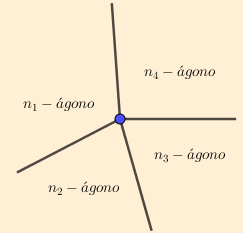
\includegraphics[width=200bp]{ladrilhamento23}
\caption{Arranjo de 4 polígonos ao redor de um vértice.}
\label{lad_tp5}
\end{figure}

As possíveis combinações de quatro polígonos regulares ao redor do vértice corresponde a determinar as soluções inteiras e positivas da equação:

\begin{equation*}
180^{\circ}\left(1-\frac{2}{n_1}\right)+180^{\circ}\left(1-\frac{2}{n_2}\right)+180^{\circ}\left(1-\frac{2}{n_3}\right)+180^{\circ}\left(1-\frac{2}{n_4}\right)=360^{\circ},
\end{equation*}

que equivale a

\begin{equation*}
\frac{1}{n_1}+\frac{1}{n_2}+\frac{1}{n_3}+\frac{1}{n_4}=1
\end{equation*}

Aplicando uma técnica de análise similar a anterior, é possível verificar que as únicas soluções inteiras e positivas dessa última equação, com $3\leq n_1\leq n_2 \leq n_3 \leq n_4$, são as seguintes

\begin{table}[H]
\centering
\setlength\tabcolsep{5mm}
\begin{tabular}{|c|c|c|c|}
\hline
\tcolor{$\bm{n_1}$} & \tcolor{$\bm{n_2}$} & \tcolor{$\bm{n_3}$} & \tcolor{$\bm{n_4}$} \\
\hline
$3$ & $3$ & $4$ & $12$ \\
\hline
$3$ & $3$ & $6$ & $6$ \\
\hline
$3$ & $4$ & $4$ & $6$ \\
\hline
$4$ & $4$ & $4$ & $4$ \\
\hline
\end{tabular}
\end{table}

Usando procedimentos semelhantes, determinamos que a classificação das possíveis combinações de $k=5$ polígonos regulares em torno de um vértice de modo que não haja nem lacunas nem sobreposições corresponde a determinação das soluções inteiras e positivas da equação

\begin{equation*}
180^{\circ}\left(1-\frac{2}{n_1}\right)+180^{\circ}\left(1-\frac{2}{n_2}\right)+180^{\circ}\left(1-\frac{2}{n_3}\right)+180^{\circ}\left(1-\frac{2}{n_4}\right)+180^{\circ}\left(1-\frac{2}{n_5}\right)=360^{\circ},
\end{equation*}

que equivale a 

\begin{equation*}
\frac{1}{n_1}+\frac{1}{n_2}+\frac{1}{n_3}+\frac{1}{n_4}+\frac{1}{n_5}=\frac{3}{2}.
\end{equation*}

As únicas soluções inteiras e positivas dessa equação, com $3\leq n_2 \leq n_3 \leq n_4 \leq n_5$, estão descritas na tabela

\begin{table}[H]
\centering
\setlength\tabcolsep{5mm}
\begin{tabular}{|c|c|c|c|c|}
\hline
\tcolor{$\bm{n_1}$} & \tcolor{$\bm{n_2}$} & \tcolor{$\bm{n_3}$} & \tcolor{$\bm{n_4}$} & \tcolor{$\bm{n_5}$} \\
\hline
$3$ & $3$ & $3$ & $3$ & $6$ \\
\hline
$3$ & $3$ & $3$ & $4$ & $4$ \\
\hline
\end{tabular}
\end{table}

Finalmente, considerando $k=6$ polígonos regulares ao redor de um vértice, temos que determinar as soluções inteiras e positivas da equação

\begin{equation*}
\frac{1}{n_1}+\frac{1}{n_2}+\frac{1}{n_3}+\frac{1}{n_4}+\frac{1}{n_5}+\frac{1}{n_6}=2,
\end{equation*}

cuja única solução é $n_1=n_2=n_3=n_4=n_5=n_6=3$

Resumindo, as possíveis combinações de polígonos regulares que podem ser arranjados em torno de um vértice a modo de cobrir o espaço ao redor dele sem lacunas nem estão dispostas na tabela:

\setlength\tabcolsep{5mm}
\begin{longtable}{|c|c|c|c|c|c|c|}
\hline\endfirsthead
\tcolor{$\bm{n_1}$} & \tcolor{$\bm{n_2}$} & \tcolor{$\bm{n_3}$} & \tcolor{$\bm{n_4}$}& \tcolor{$\bm{n_5}$} & \tcolor{$\bm{n_6}$} & \tcolor{Configuração} \\
\hline
$3$ & $7$ & $42$ & & & & $3-7-42$ \\
\hline
$3$ & $8$ & $24$ & & & & $3-8-24$ \\
\hline
$3$ & $9$ & $18$ & & & & $3-9-18$ \\
\hline
$3$ & $10$ & $15$ & & & & $ 3-10-15$ \\
\hline
$3$ & $12$ & $12$ & & & & $3-12-12$ \\
\hline
$4$ & $5$ & $20$ & & & & $4-5-20$ \\
\hline
$4$ & $6$ & $12$ & & & & $4-6-12$ \\
\hline
$4$ & $8$ & $8$ & & & & $4-8-8$ \\
\hline
$5$ & $5$ & $10$ & & & & $5-5-10$ \\
\hline
$6$ & $6$ & $6$ & & & & $6-6-6$ \\
\hline
$3$ & $3$ & $4$ & $12$ & & & $3-3-4-12$ \\
\hline
$3$ & $3$ & $6$ & $6$ & & & $3-3-6-6$ \\
\hline
$3$ & $4$ & $4$ & $6$ & & & $3-4-4-6$ \\
\hline
$4$ & $4$ & $4$ & $4$ & & & $4-4-4-4$ \\
\hline
$3$ & $3$ & $3$ & $3$ & $6$ & & $3-3-3-3-6$ \\
\hline
$3$ & $3$ & $3$ & $4$ & $4$ & & $3-3-3-4-4$ \\
\hline
$3$ & $3$ & $3$ & $3$ & $3$ & $3$ & $3-3-3-3-3-3$ \\
\hline
\end{longtable}

Será que todas as  combinações /configurações que constam na tabela anterior podem ser construídas geometricamente de modo a ladrilhar o plano?

\clearpage
\def\currentcolor{session1}

\begin{objectives}{Investigando as combinações}
{
	\begin{itemize}
	\item Entender que existe uma regra geral que permite determinar quando uma certa combinação de polígonos regulares produz um ladrilhamento
	\item Criar ladrilhamentos no plano usando polígonos regulares de mais de um tipo
	\item \textbf{Conceitos abordados}: Ladrilhamentos semirregulares
	\end{itemize}
}{1}{1}
\end{objectives}
\begin{sugestions}{Investigando as combinações}
{
	\textbf{Organização em sala de aula}: Essa é uma continuação da atividade anterior. Sugerimos que as atividades sejam realizadas de forma individual ou em duplas. A reflexão mediada pela manipulação dos polígonos regulares  pode ser favorecida pela discussão com um colega. Grupos maiores podem gerar dispersão.

	\textbf{Dificuldades previstas}: A ideia é que os estudantes  tentem  montar o ladrilhamento usando as peças de cada configuração (quando possível). Se o professor não tiver as peças disponíveis, sugira que os alunos façam esboços e tentem chegar em alguma conclusão.
 
	\textbf{Enriquecimento da discussão}: Estimule os alunos a justificarem cada vez que eliminarem alguma configuração ou afirmarem que é possível realizar o ladrilhamento. Observe com os alunos que é possível construir um ladrilhamento usando triângulos equiláteros, quadrados e dodecágonos regulares, mas a distribuição de ladrilhos ao redor de cada vértice não será sempre a mesma. Questione os  alunos que quando um ladrilhamento como queremos é possível,  se a sequência dos polígonos regulares  ao redor de cada vértice é sempre a mesma, em ambos os sentidos. Observe que esse fato é o  que ocorre com a configuração 3-6-3-6.  Apesar de ser possível construir um vértice do tipo 3-3-6-6 não é possível manter em um ladrilhamento todos os vértices com este mesmo tipo. Questione aos alunos se isso é um problema.

	\textbf{Material necessário}: Polígonos regulares do encarte.
}{1}{1}
\end{sugestions}
\begin{answer}{Investigando as combinações}
{
	Todas as respostas para as questões realizadas na atividade encontram-se no organizando.
}{1}
\end{answer}

\explore{Ladrilhamentos semirregulares} \label{at_ladsemi}

\begin{task} {Investigando as combinações}

\textbf{Parte 1:} Considerando as  combinações obtidas para $k=3$.
 
\begin{table}[H]
\centering
\setlength\tabcolsep{5mm}
\begin{tabular}{|c|c|c|c|}
\hline
\tcolor{$\bm{n_1}$} & \tcolor{$\bm{n_2}$} & \tcolor{$\bm{n_3}$} &  \tcolor{Configuração} \\
\hline
$3$ & $7$ & $42$ & $3-7-42$ \\
\hline
$3$ & $8$ & $24$ &  $3-8-24$ \\
\hline
$3$ & $9$ & $18$ &  $3-9-18$ \\
\hline
$3$ & $10$ & $15$ &  $ 3-10-15$ \\
\hline
$3$ & $12$ & $12$ &  $3-12-12$ \\
\hline
$4$ & $5$ & $20$ &  $4-5-20$ \\
\hline
$4$ & $6$ & $12$ &  $4-6-12$ \\
\hline
$4$ & $8$ & $8$ &  $4-8-8$ \\
\hline
$5$ & $5$ & $10$ &  $5-5-10$ \\
\hline
$6$ & $6$ & $6$ &  $6-6-6$ \\
\hline
\end{tabular}
\end{table}

\begin{enumerate}

\item	Com quais delas é possível realizar um ladrilhamento no plano? Justifique?
\item	Justifique por que com algumas dessas combinações não é possível ladrilhar o plano.

\end{enumerate}

\textbf{Parte 2:} Considerando as  combinações obtidas para $k=4$. 

\begin{table}[H]
\centering
\setlength\tabcolsep{5mm}
\begin{tabular}{|c|c|c|c|c|}
\hline
\tcolor{$\bm{n_1}$} & \tcolor{$\bm{n_2}$} & \tcolor{$\bm{n_3}$} & \tcolor{$\bm{n_4}$}&  \tcolor{Configuração} \\
\hline

$3$ & $3$ & $4$ & $12$ & $3-3-4-12$ \\
\hline
$3$ & $3$ & $6$ & $6$ &  $3-3-6-6$ \\
\hline
$3$ & $4$ & $4$ & $6$ & $3-4-4-6$ \\
\hline
$4$ & $4$ & $4$ & $4$ &  $4-4-4-4$ \\
\hline
\end{tabular}
\end{table}

Observe que ao dispor os polígonos regulares ao redor de um vértice podemos obter configurações distintas (\hyperref[ladreg1]{figura \ref{ladreg1}}).

\begin{figure}[H]
\centering
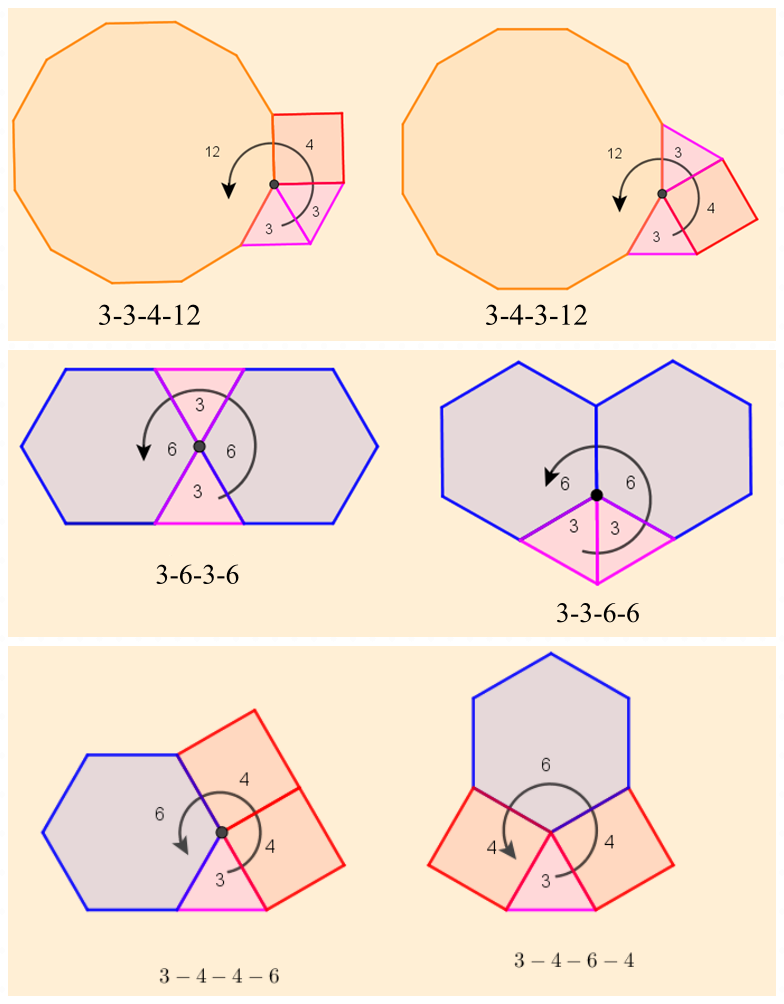
\includegraphics[width=250bp]{ladreg1}
\caption{Arranjo de 4 polígonos regulares ao redor de um vértice.}
\label{ladreg1}
\end{figure}

\begin{enumerate}
\item Justifique por que elas são diferentes? 
\item Com quais delas é possível ladrilhar o plano? Justifique!

\end{enumerate}

\textbf{Parte 3:} Considerando as  combinações obtidas para $k=5$ e $k=6$.

\setlength\tabcolsep{5mm}
\begin{longtable}{|c|c|c|c|c|c|c|}
\hline\endfirsthead
\tcolor{$\bm{n_1}$} & \tcolor{$\bm{n_2}$} & \tcolor{$\bm{n_3}$} & \tcolor{$\bm{n_4}$} & \tcolor{$\bm{n_5}$} & \tcolor{$\bm{n_6}$} & \tcolor{Configuração} \\
\hline
$3$ & $3$ & $3$ & $3$ & $6$ & & $3-3-3-3-6$ \\
\hline
$3$ & $3$ & $3$ & $4$ & $4$ & & $3-3-3-4-4$ \\
\hline
$3$ & $3$ & $3$ & $3$ & $3$ & $3$ & $3-3-3-3-3-3$ \\
\hline
\end{longtable}

Com quais delas é possível ladrilhar o plano? Justifique!

\textbf{Parte 4:}
Observe a tabela e responda:

\setlength\tabcolsep{5mm}
\begin{longtable}{|c|c|c|c|c|c|c|}
\hline\endfirsthead
\tcolor{$\bm{n_1}$} & \tcolor{$\bm{n_2}$} & \tcolor{$\bm{n_3}$} & \tcolor{$\bm{n_4}$} & \tcolor{$\bm{n_5}$} & \tcolor{$\bm{n_6}$} & \tcolor{Configuração} \\
\hline
$3$ & $7$ & $42$ & & & & $3-7-42$ \\
\hline
$3$ & $8$ & $24$ & & & & $3-8-24$ \\
\hline
$3$ & $9$ & $18$ & & & & $3-9-18$ \\
\hline
$3$ & $10$ & $15$ & & & & $ 3-10-15$ \\
\hline
$3$ & $12$ & $12$ & & & & $3-12-12$ \\
\hline
$4$ & $5$ & $20$ & & & & $4-5-20$ \\
\hline
$4$ & $6$ & $12$ & & & & $4-6-12$ \\
\hline
$4$ & $8$ & $8$ & & & & $4-8-8$ \\
\hline
$5$ & $5$ & $10$ & & & & $5-5-10$ \\
\hline
$6$ & $6$ & $6$ & & & & $6-6-6$ \\
\hline
$3$ & $3$ & $4$ & $12$ & & & $3-3-4-12$ \\
\hline
$3$ & $3$ & $6$ & $6$ & & & $3-3-6-6$ \\
\hline
$3$ & $4$ & $4$ & $6$ & & & $3-4-4-6$ \\
\hline
$4$ & $4$ & $4$ & $4$ & & & $4-4-4-4$ \\
\hline
$3$ & $3$ & $3$ & $3$ & $6$ & & $3-3-3-3-6$ \\
\hline
$3$ & $3$ & $3$ & $4$ & $4$ & & $3-3-3-4-4$ \\
\hline
$3$ & $3$ & $3$ & $3$ & $3$ & $3$ & $3-3-3-3-3-3$ \\
\hline
\end{longtable}

Quais as configurações que produzem ladrilhamentos do plano?


\end{task}

\arrange{Ladrilhamentos semirregulares}

Na primeira parte da \hyperref[at_ladsemi]{atividade \ref{at_ladsemi}} solicitamos investigar quais das dez possíveis combinações de 3 polígonos regulares, definiam um ladrilhamento semirregular. 
Vamos começar nossa investigação considerando uma combinação de três polígonos $3-n_2-n_3$, dos quais um é um triângulo regular($n_1=3$). 
Nessa configuração, $3$ se refere a um triângulo equilátero, $n_2$ e $n_3$ são polígonos regulares com quantidade $n_2$ e $n_3$ de lados, respectivamente. Os comprimentos das arestas de todos os polígonos regulares usados são iguais. Para produzir um ladrilhamento, o triângulo equilátero deve ter a mesma configuração  de polígonos regulares em todos os seus três vértices; ou seja, eles devem ser "rodeados" por polígonos regulares da mesma maneira. A \hyperref[semi1]{figura \ref{semi1}} ilustra essa situação.  
 
\begin{figure}[H]
\centering
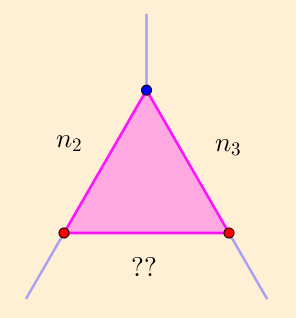
\includegraphics[width=150bp]{semi1}
\caption{Combinação de polígonos regulares ao redor do vértice de um triângulo equilátero.}
\label{semi1}
\end{figure}

Na \hyperref[semi1]{figura \ref{semi1}}, os polígonos regulares  $n_2$ e $n_3$ estão dispostos para completar o vértice azul. No entanto, os vértices vermelhos serão completados apenas quando o polígono regular em "$??$" for $n_2$ ou $n_3$. Portanto, a única maneira de fazer isso é definindo $n_2 = n_3$. Isso significa que o padrão se torna $3-n_2- n_2$. 
Isso elimina as configurações $3-7-42$, $3-8-24$, $3-9-18$ e $3-10-15$. Logo, existe apenas uma combinação, $3-12-12$, com a qual se permite um ladrilhamento do plano (\hyperref[semi2]{figura \ref{semi2}})

\begin{figure}[H]
\centering
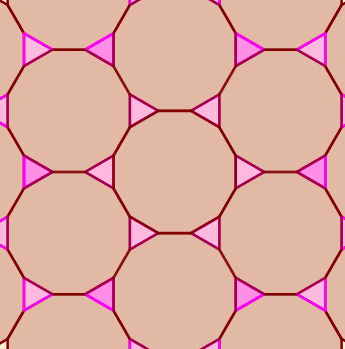
\includegraphics[width=150bp]{semi2}
\caption{Ladrilhamento produzido a partir da configuração $3-12-12$.}
\label{semi2}
\end{figure}

O mesmo argumento vale para todos os polígonos com quantidade ímpar de lados, que devem ser combinados com outros dois outros polígonos regulares (\hyperref[semi3]{figura \ref{semi3}}). Isso elimina as combinações $4-5-20$ (leia-o como $5-20-4$) e $5-5-10$.


\begin{figure}[H]
\centering
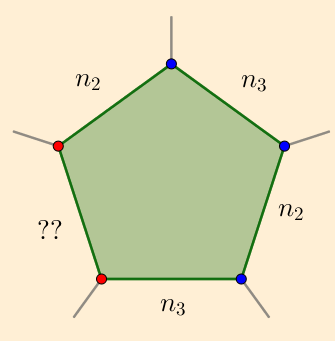
\includegraphics[width=150bp]{semi3}
\caption{Combinação de polígonos ao redor do vértice de um pentágono regular.}
\label{semi3}
\end{figure}

Pensando nas combinações de três polígonos regulares  ($3-n_2-n_3$), dos quais um é um quadrado. A  configuração seria $4-n_2-n_3$. A \hyperref[semi4]{figura \ref{semi4}} ilustra que existem apenas duas maneiras nas quais a configuração $4-n_2-n_3$ se estenderia, mantendo a mesma configuração de polígonos regulares em todos os vértices. 

\begin{figure}[H]
\centering
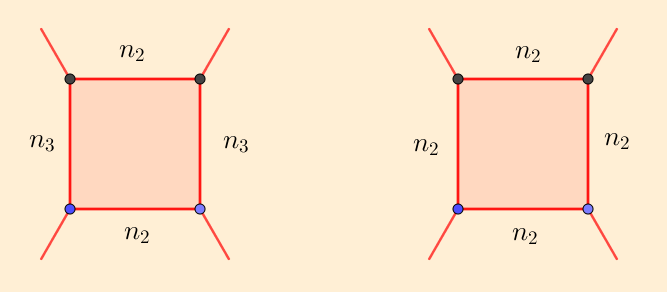
\includegraphics[width=300bp]{semi4}
\caption{Combinação de polígonos regulares ao redor do vértice de um quadrado.}
\label{semi4}
\end{figure}

Nesse caso ou $n_2= n_3$ ou $n_2$ e $n_3$ são colocados alternadamente ao redor do vértice. Isso qualifica as combinações $4-8-8$ e $4-6-12$ como ladrilhamentos semirregulares (\hyperref[semi5]{figura \ref{semi5}}).

\begin{figure}[H]
\centering
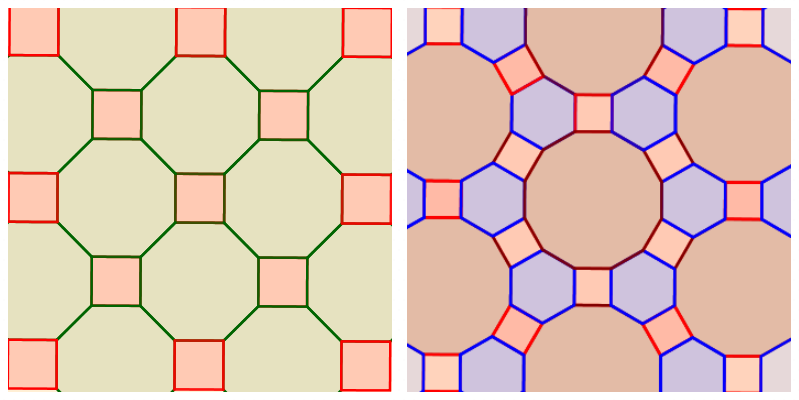
\includegraphics[width=300bp]{semi5}
\caption{Ladrilhamentos nas configurações $4-8-8$ e $4-6-12$.}
\label{semi5}
\end{figure}

Obviamente a configuração $6-6-6$ também produz um ladrilhamento, que é o ladrilhamento regular feito com hexágonos, como já visto.

Resumindo, existem apenas quatro ladrilhamentos usando três polígonos regulares
ao redor de um vértice, e estes tem as seguintes configurações  $3-12-12$, $4-8-8$,  $4-6-12$  e $6-6-6$.

Na parte 2 da \hyperref[at_ladsemi]{atividade \ref{at_ladsemi}} consideramos as combinações obtidas quando usamos  4 polígonos regulares. 
Vamos investigar o que ocorre quando ao redor de um vértice se tivermos  dois triângulos equiláteros e outros dois polígonos regulares, ou seja uma configuração do tipo $3-3-n_3-n_4$. Esses polígonos regulares podem ser organizados como $3-3-n_3-n_4$ ou $3-n_3-3-n_4$. 
Começaremos nossa investigação colocando os polígonos regulares $n_3$ e $n_4$ no vértice azul (\hyperref[semi6]{figura \ref{semi6}}). 


\begin{figure}[H]
\centering
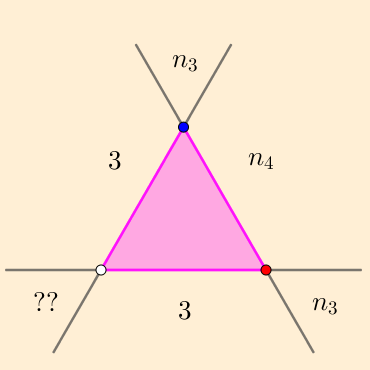
\includegraphics[width=150bp]{semi6}
\caption{Combinação de polígonos regulares ao redor de um vértice de um triângulo equilátero.}
\label{semi6}
\end{figure}


Nesse caso, a configuração dos polígonos regulares em torno do vértice azul seria $3-3-n_3-n_4$. Para ter a mesma configuração no vértice vermelho, os polígonos regulares devem ser organizados no sentido contrário. No vértice branco, entretanto, haverá três triângulos equiláteros, perfazendo a soma total dos ângulos internos como $180^{\circ}$, não deixando nenhuma possibilidade de encaixar qualquer outro polígono. 

Portanto, configurações do tipo $3-3-n_3-n_4$ não produzem um ladrilhamento semirregular. Isso mostra a impossibilidade das configurações $3-3-4-12$ e $3-3-6-6$.

A outra possibilidade é um  arranjo do tipo $3-n_3-3-n_4$, ao redor do vértice azul, como ilustra a \hyperref[semi7]{figura \ref{semi7}}.



\begin{figure}[H]
\centering
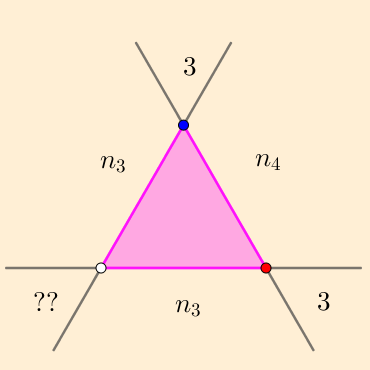
\includegraphics[width=150bp]{semi7}
\caption{Combinação de polígonos ao redor de um vértice de um triângulo equilátero.}
\label{semi7}
\end{figure}

Observamos que para manter a mesma configuração no vértice branco, os polígonos regulares com quantidade de lados  $n_3$  e $n_4$ teriam que ser iguais. Assim, a configuração $3-3-4-12$ (dois triângulos equiláteros, um quadrado e um dodecágono regular) não produzirá um ladrilhamento. Porém, a combinação $3-3-6-6$ quando reorganizada como $3-6-3-6$ produzirá um ladrilhamento semirregular (\hyperref[semi8]{figura \ref{semi8}}).



\begin{figure}[H]
\centering
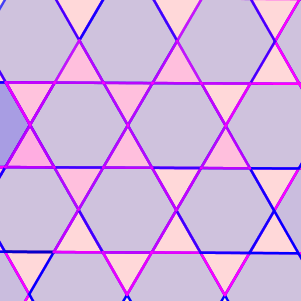
\includegraphics[width=150bp]{semi8}
\caption{Ladrilhamento na configuração $3-6-3-6$.}
\label{semi8}
\end{figure}

Fazendo um raciocínio semelhante, podemos concluir que a combinação $3-4-4-6$ não produz um ladrilhamento semirregular. No entanto, se os polígonos regulares forem reorganizados como $3-4-6-4$ então, é possível produzir um ladrilhamento semirregular, como ilustra a \hyperref[semi9]{figura \ref{semi9}}.

\begin{figure}[H]
\centering
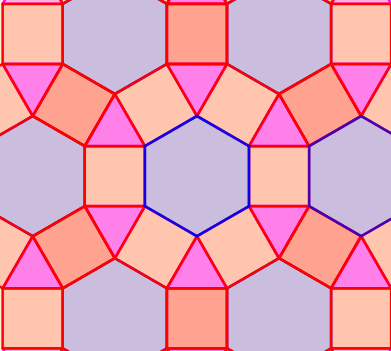
\includegraphics[width=150bp]{semi9}
\caption{Ladrilhamento na configuração $3-4-6-4$.}
\label{semi9}
\end{figure}


E obviamente, a configuração $4-4-4-4$ produz o ladrilhamento regular formado apenas por quadrados, conforme foi visto anteriormente.

A terceira parte da \hyperref[at_ladsemi]{atividade \ref{at_ladsemi}}, tinha como objetivo investigar as combinações com 5 e 6 polígonos regulares ao redor de um vértice.

A combinação para 6 polígonos $3-3-3-3-3-3$ produz o ladrilhamento regular formado por triângulos equiláteros.

Ainda restam duas configurações de 5 polígonos regulares. Vamos  considerá-las separadamente. A configuração $3-3-3-4-4$, também pode ser arranjada como  $3-3- 4-3-4$. A \hyperref[semi10]{figura \ref{semi10}} ilustra um arranjo em torno do vértice de um triângulo equilátero para ambas configurações.

\begin{figure}[H]
\centering
\includegraphics[width=300bp]{semi10}
\caption{Combinação de polígonos regulares ao redor de um vértice de um triângulo equilátero.}
\label{semi10}
\end{figure}

Observamos que é possível criar ladrilhamentos semirregulares para as configurações  $3-3-3-4-4$ e $3-3-4-3-4$ (\hyperref[semi11]{figura \ref{semi11}}).

\begin{figure}[H]
\centering
\includegraphics[width=300bp]{semi11}
\caption{Ladrilhamentos semirregulares para as configurações  $3-3-3-4-4$ e $3-3-4-3-4$.}
\label{semi11}
\end{figure}

 

E, finalmente, a \hyperref[semi12]{figura \ref{semi12}} ilustra o ladrilhamento produzido pela configuração $3-3-3-3-6$.


\begin{figure}[H]
\centering
\includegraphics[width=150bp]{semi12}
\caption{Ladrilhamento produzido pela configuração 3-3-3-3-6.}
\label{semi12}
\end{figure}


\clearpage
A tabela a seguir ilustra um resumo das configurações apresentadas.


\setlength\tabcolsep{3.5mm}
\begin{longtable}{|c|c|c|c|c|c|c|c|c}
\hline\endfirsthead
\tcolor{$\bm{n_1}$} & \tcolor{$\bm{n_2}$} & \tcolor{$\bm{n_3}$} & \tcolor{$\bm{n_4}$}& \tcolor{$\bm{n_5}$} & \tcolor{$\bm{n_6}$} & \tcolor{Configuração} & \tcolor{\makecell{Ladrilha \\ o plano}} \\
\hline
$3$ & $7$ & $42$ & & & & $3-7-42$ & Não\\
\hline
$3$ & $8$ & $24$ & & & & $3-8-24$ & Não\\
\hline
$3$ & $9$ & $18$ & & & & $3-9-18$ & Não\\
\hline
$3$ & $10$ & $15$ & & & & $ 3-10-15$ & Não\\
\hline
\titem{$\bm{3}$} & \titem{$\bm{12}$} & \titem{$\bm{12}$} & & & & \titem{$\bm{3-12-12}$} & \titem{Sim}\\
\hline
$4$ & $5$ & $20$ & & & & $4-5-20$ & Não\\
\hline
\titem{$\bm{4}$} & \titem{$\bm{6}$} & \titem{$\bm{12}$} & & & & \titem{$\bm{4-6-12}$} & \titem{Sim}\\
\hline
\titem{$\bm{4}$} & \titem{$\bm{8}$} & \titem{$\bm{8}$} & & & & \titem{$\bm{4-8-8}$} & \titem{Sim}\\
\hline
$5$ & $5$ & $10$ & & & & $5-5-10$ & Não\\
\hline
\titem{$\bm{6}$} & \titem{$\bm{6}$} & \titem{$\bm{6}$} & & & & \titem{$\bm{6-6-6}$} & \titem{Sim}\\
\hline
$3$ & $3$ & $4$ & $12$ & & & $3-3-4-12$ & Não\\
\hline
\titem{$\bm{3}$} & \titem{$\bm{3}$} & \titem{$\bm{6}$} & \titem{$\bm{6}$} & & & \titem{$\bm{3-3-6-6}$} & \titem{Sim}\\
\hline
\titem{$\bm{3}$} & \titem{$\bm{4}$} & \titem{$\bm{4}$} & \titem{$\bm{6}$} & & & \titem{$\bm{3-4-4-6}$} & \titem{Sim}\\
\hline
\titem{$\bm{4}$} & \titem{$\bm{4}$} & \titem{$\bm{4}$} & \titem{$\bm{4}$} & & & \titem{$\bm{4-4-4-4}$} & \titem{Sim}\\
\hline
\titem{$\bm{3}$} & \titem{$\bm{3}$} & \titem{$\bm{3}$} & \titem{$\bm{3}$} & \titem{$\bm{6}$} & & \titem{$\bm{3-3-3-3-6}$} & \titem{Sim}\\
\hline
\titem{$\bm{3}$} & \titem{$\bm{3}$} & \titem{$\bm{3}$} & \titem{$\bm{4}$} & \titem{$\bm{4}$} & & \titem{$\bm{3-3-3-4-4}$} & \titem{Sim}\\
\hline
\titem{$\bm{3}$} & \titem{$\bm{3}$} & \titem{$\bm{3}$} & \titem{$\bm{3}$} & \titem{$\bm{3}$} & \titem{$\bm{3}$} & \titem{$\bm{3-3-3-3-3-3}$} & \titem{Sim}\\
\hline
\end{longtable}

A \hyperref[semit]{figura \ref{semit}} ilustra todos os ladrilhamentos semirregulares.


\begin{figure}[H]
\centering
\includegraphics[width=400bp]{semit}
\caption{Ladrilhamentos semirregulares.}
\label{semit}
\end{figure}

Ou seja, acabamos de mostrar que existem exatamente 11 maneiras de  cobrir o plano utilizando-se exclusivamente polígonos regulares sujeitos as seguintes condições:
\begin{itemize}
\item se dois polígonos regulares intersectam-se, então essa interseção é um lado ou um vértice comum.
\item A distribuição dos polígonos regulares ao redor de cada vértice é sempre a mesma.
\end{itemize}

%%%%%%%%%%%%%%%


\cleardoublepage
\def\currentcolor{session1}
%\begin{texto}
{
%\paragraph {Objetivo geral da seção}
%Reconhecer que existem outros ladrilhamentos, como os aperiódicos e os que não são do tipo lado a lado.}
%\end{texto}
\begin{objectives}{Ladrilhando com retângulos}
{
	\begin{itemize}
	\item Reconhecer ladrilhamentos que não são do tipo lado a lado.
	\item \textbf{Conceitos abordados}: Ladrilhamentos monoédricos.
	\end{itemize}	
}{1}{1}
\end{objectives}
\begin{sugestions}{Ladrilhando com retângulos}
{
	\textbf{Organização em sala de aula}: A atividade pode ser feita em duplas, para que os alunos possam discutir com o colega os ladrilhamentos que serão construídos.

	\textbf{Dificuldades previstas}: Nesta atividade, o aluno deverá construir um ladrilhamento que não é o usual ( lado a lado). É possível que inicialmente os alunos tenham alguma dificuldade, pois deverão quebrar as regras estabelecidas. Ou seja, poderão construir ladrilhamentos onde existem arestas que não são comuns a dois polígonos.

	\textbf{Enriquecimento da discussão}: Observe com os alunos que esse tipo de ladrilho é muito comum no revestimento do tipo parquet. Faça-os perceber que existem vários designs possíveis no momento que não existe mais a necessidade das arestas dos polígonos serem comuns. 

	\textbf{Material necessário}: lápis e papel

}{1}{1}
\end{sugestions}
\begin{answer}{Ladrilhando com retângulos}
{
	\begin{enumerate}
	\item Qualquer um desses padrões, por exemplo:
	\begin{figure}[H]
	\centering
	\includegraphics[width=.5\linewidth]{reviso6}
	\end{figure}
	\end{enumerate}
}{1}
\end{answer}
\begin{objectives}{Ladrilhamento do tipo Penrose}
{
	\begin{itemize}
	\item Reconhecer ladrilhamentos do tipo Penrose.
	\item \textbf{Conceitos abordados}: ladrilhamentos com polígonos irregulares.
	\end{itemize}
}{1}{2}
\end{objectives}
\begin{sugestions}{Ladrilhamento do tipo Penrose}
{
	\textbf{Organização em sala de aula}: A atividade pode ser feita em duplas, para que os alunos possam discutir com o colega os ladrilhamentos que serão construídos.

	\textbf{Dificuldades}: A primeira dificuldade poderá ser a construção das peças, pois será necessário usar um pentágono regular. Para facilitar o processo,  as peças ( pipa e flecha) fazem parte do encarte, oriente seus alunos a utilizarem-no. Acredita-se também que o aluno possa ter dificuldade em ladrilhar o plano com as formas, pois poderá fazer um ladrilhamento do tipo não periódico, que é diferente do que já estava sendo apresentado. 

	\textbf{Enriquecimento da discussão}: Faça os alunos perceberem  que existem vários designs possíveis usando essas duas peças, porém a maioria produzirá ladrilhamentos que não são periódicos. Questione os alunos sobre o tipo de transformação usada, fazendo questionamento do tipo: você usou translações, rotações ou reflexões para criar seu design? Você usou uma combinação de transformações? 

	\textbf{Material necessário}: Polígono impresso do encarte, tesoura, cola, lápis de cor.
}{1}{2}
\end{sugestions}
\begin{answer}{Ladrilhamento do tipo Penrose}
{
	\begin{enumerate}
	\item ---
	\item Translações e rotações, por exemplo.
	\item Não periódico e feitos com um ladrilho não convexo.
	\end{enumerate}
}{1}
\end{answer}
\clearmargin
\begin{objectives}{Um ladrilhamento no estilo Escher}
{
	\begin{itemize}
	\item Utilizar transformações geométricas para construir ladrilhamentos.
	\item Entender que é necessário utilizar polígonos regulares e transformações geométricas para construir ladrilhamentos do tipo Escher.
	\item \textbf{Conceitos abordados}: transformações e ladrilhamentos.
	\end{itemize}
}{1}{1}
\end{objectives}
\begin{sugestions}{Um ladrilhamento no estilo Escher}
{
	\textbf{Organização em sala de aula}: Essa atividade foi planejada para ser realizada de forma individual. 

	\textbf{Dificuldades previstas}: Nesta atividade, o aluno deverá construir um  ladrilhamento começando com um polígono regular , mas fazendo alterações no seu formato.  Acreditamos que se o aluno seguir as orientações, não terá dificuldade em realizar a atividade. Caso prefira usar um software para realizar essa atividade, recomenda-se olhar o vídeo https://youtu.be/zZ2wrNdYchw que indica um aplicativo interessante para esse tipo de construção.  

	\textbf{Enriquecimento da discussão}: lembre aos alunos que no início do capítulo trabalhamos com um ladrilhamento utilizando lagartos. A técnica que o artista que inventou aquele ladrilhamento é a mesma que estamos utilizando essa atividade. 

	\textbf{Material necessário}: Polígono impresso do encarte, tesoura, cola, lápis de cor
}{1}{1}
\end{sugestions}
\begin{answer}{Um ladrilhamento no estilo Escher}
{
	Resposta pessoal.
}{1}
\end{answer}


\explore{Outros ladrilhamentos}



\begin{task}{Ladrilhando com retângulos} \label{at_outros1}

Os pisos de algumas casa são cobertos por ladrilhos retangulares. O padrão ilustrado na \hyperref[peixe]{figura \ref{peixe}} é denominado espinha de peixe. 

	\begin{figure}[H]
	\centering
	\includegraphics[width=250bp]{ladrilhamento16}
	\caption{Ladrilhamento tipo espinha de peixe. Fonte: \href{http://www.tilehomeguide.com/tile-patterns-the-ultimate-quick-read-beginners-guide-including-secrets-of-tile-professionals-revealed/}{The Tile Home Guide}}
	\label{peixe}
	\end{figure}

 Em papel quadriculado, crie dois ladrilhamentos  diferentes a partir de ladrilhos retangulares congruentes.

\end{task}
\clearpage
\begin{task}{Ladrilhamento do tipo Penrose}\label{at_outros2}

Parte do hall central do departamento de Matemática e Ciência da Computação no Carlton College em Minessota nos Estados Unidos, usa ladrilhos do tipo Penrose (\hyperref[pen1]{figura \ref{pen1}}). Esses ladrilhos foram inventados pelo matemático inglês Roger Penrose na década de 1970.

\begin{figure}[H]
	\centering
	\includegraphics[width=230bp]{reviso8}
	\caption{Padrão de Pavimento do Carleton College. Fonte: Adaptado de  \href{https://www.math.carleton.edu/penrose/index.html} {Carleton} }
	\label{pen1}
\end{figure}

Observe que os ladrilhos têm em duas formas diferentes, a pipa e a flecha. Esses quadriláteros podem ser construídos a partir de um pentágono regular, como ilustra a \hyperref[pen2]{figura \ref{pen2}}.

	\begin{figure}[H]
	\centering
	\includegraphics[width=230bp]{ladrilhamento52}
	\caption{Pipa e Flecha}
	\label{pen2}
	\end{figure}
	
	\begin{enumerate}
			\item Copie as formas da pipa e da flecha ( no encarte) em um papel de gramatura mais alta. Recorte-as e crie dois ladrilhamentos diferentes.
		\item Escreva um breve parágrafo explicando quais transformações geométricas você usou para criar o ladrilhamento no item anterior desta atividade. 
		\item O que os ladrilhamentos construídos nessa atividade possuem de diferente dos ladrilhamentos construídos anteriormente?
	\end{enumerate}
	
\end{task}


\begin{task}{Um ladrilhamento no estilo Escher}\label{at_outros3}
\begin{enumerate}
\item Vamos usar um triângulo equilátero para compor um ladrilhamento no estilo Escher, para isso:  
\begin{enumerate}

	\item Desenhe um triângulo equilátero em um papel. Recorte-o  cole-o em uma folha de papel de gramatura alta para construção. Recorte o triângulo novamente.

	\item Dentro do triângulo, desenhe uma curva que conecta dois vértices adjacentes. Corte ao longo da curva para remover uma parte do triângulo (que vamos denominar peça), como ilustra a \hyperref[escher1]{figura \ref{escher1}}.

	\begin{figure}[H]
	\centering
	\includegraphics[width=350bp]{ladrilhamento42}
	\caption{Instruções para realizar o ladrilhamento.}
	\label{escher1}
	\end{figure}

	\item Gire a peça que você removeu $60^{\circ}$ no sentido anti-horário sobre o vértice da extremidade superior da curva desenhada. Mova a peça para o outro lado do triângulo. Cole-a para completar seu ladrilho, como ilustra a \hyperref[escher2]{figura \ref{escher2}}.

	\begin{figure}[H]
	\centering
	\includegraphics[width=350bp]{ladrilhamento43}
	\caption{Instruções para realizar o ladrilhamento.}
	\label{escher2}
	\end{figure}

	\item Para ladrilhar o plano, utilizando o lápis, faça um traço ao redor do ladrilho. Em seguida, gire e desenhe o ladrilho repetidamente até que se tenha o design pretendido.
	\item Adicione cores e desenhos ao ladrilho para que pareça uma obra de arte, como ilustra a \hyperref[escher3]{figura \ref{escher3}}.

	\begin{figure}[H]
	\centering
	\includegraphics[width=200bp]{ladrilhamento44}
	\caption{Ladrilhamento parcial.}
	\label{escher3}
	\end{figure}
\end{enumerate}

	\item Repita as etapas de i) a v) usando um paralelogramo e translações, para criar outro ladrilhamento no estilo Escher.

\end{enumerate}
\end{task}



\clearpage
\arrange{Outros ladrilhamentos}


Na primeira seção desse capítulo, vimos que qualquer triângulo e qualquer quadrilátero ladrilham o plano, alguns pentágonos e hexágonos também o fazem. Além disso, exploramos ladrilhamentos semirregulares. 

Nas atividades anteriores (\ref{at_outros1} e \ref{at_outros2}) exploramos um pouco mais sobre os ladrilhamentos usando polígonos, mas dessa vez, consideramos alguns polígonos bem especiais. A \hyperref[at_outros1]{atividade \ref{at_outros1}} tratou de ladrilhamentos usando ladrilhos retangulares.

Esse tipo de ladrilhamento é muito comum em  paredes e pisos revestidos com peças denominadas \textit{Subway Tiles }(azulejo de metrô). Construtores e arquitetos  há muito exploram diferentes maneiras de arranjar esses azulejos por razões estruturais e estéticas. Do ponto de vista  matemático, são interessantes como exemplos de ladrilhamentos que (em geral) não são  lado a lado, ou seja, existem arestas que não são comuns a dois polígonos, como ilustra a \hyperref[lad_ret1]{figura \ref{lad_ret1}}.

\begin{figure}[H]
	\centering
	\includegraphics[width=400bp]{lad_ret_1}
	\caption{Exemplos de ladrilhamentos.}
	\label{lad_ret1}
	\end{figure}


A \hyperref[lad_ret]{figura \ref{lad_ret}} ilustra exemplos de como os retângulos podem ser arranjados de forma realizar uma pavimentação.
 \begin{figure}[H]
	\centering
	\includegraphics[width=300bp]{lad_ret}
	\caption{Exemplos de ladrilhamentos.}
	\label{lad_ret}
	\end{figure}

A \hyperref[at_outros2]{atividade \ref{at_outros2}} tratou de ladrilhos especiais que são construídos a partir de um pentágono regular. Essas peças são ditas especiais pois são constituídas por triângulos denominados áureos. De fato, considerando  um pentágono $ABCDE$ de lado unitário, sabemos que cada um dos ângulos internos desse polígono mede $108^{\circ}$ (\hyperref[penr_9]{figura \ref{penr_9}}). 

\begin{figure}[H]
	\centering
	\includegraphics[width=150bp]{penr9}
	\caption{Medida do ângulo interno de um pentágono regular.}
	\label{penr_9}
	\end{figure}


Como as diagonais de um polígono regular dividem os ângulos internos em partes congruentes, no caso do pentágono regular, cada ângulo interno é dividido via duas diagonais. Logo o ângulo de  $108^{\circ}$ é dividido em três ângulos de $36^{\circ}$(\hyperref[penr_10]{figura \ref{penr_10}}). 


\begin{figure}[H]
\centering
\includegraphics[width=150bp]{penr10}
\caption{Medida do ângulo interno de um pentágono regular.}
\label{penr_10}
\end{figure}


Seja o ponto P como a intersecção das diagonais CE e BD, segue que  o triângulo $DEP$ é isósceles (pois $\hat{E}= 36^{\circ}$, $\hat{D}=\hat{P}$) e portanto, $EP=1$ (\hyperref[penr_11]{figura \ref{penr_11}}).

\begin{figure}[H]
	\centering
	\includegraphics[width=150bp]{penr11}
	\caption{Triângulo $DEP$.}
	\label{penr_11}
\end{figure}


Fazendo $PE =x$ e considerando os triângulos $PBC$ e $BCE$, temos no triângulo $PBC$ (\hyperref[penr_12]{figura \ref{penr_12}}), os ângulos internos $P\hat{C}B$ e $B\hat{P}C$ são congruentes e medem $72^{\circ}$ e o ângulo $C\hat{B}P$ mede $36^{\circ}$. 

\begin{figure}[H]
	\centering
	\includegraphics[width=150bp]{penr12}
	\caption{Triângulo $PBC$.}
	\label{penr_12}
\end{figure}


No triângulo $BCE$, os ângulos ângulos internos $E\hat{C}B$ e $C\hat{B}E$ são congruentes e medem $72^{\circ}$ e o ângulo $B\hat{E}C$ mede $36^{\circ}$ (\hyperref[penr_13]{figura \ref{penr_13}}).


\begin{figure}[H]
	\centering
	\includegraphics[width=150bp]{penr13}
	\caption{Triângulo $BCE$.}
	\label{penr_13}
\end{figure}


Ou seja, os triângulos $PBC$ e $BCE$ são isósceles e semelhantes. Como estamos considerando $ABCDE$ unitário e  $PE = x$, segue que $EC= EB = 1+x$. E da semelhança de triângulos, resulta a seguinte equação:
$$\frac{x+1}{1}=\frac{1}{x}.$$

Cuja solução positiva é $x=\frac{sqrt{5}-1}{2}$.
Disso resulta que o ponto $P$ divide a diagonal $CE$ em média e extrema razão, ou seja, na razão áurea e por essa razão os triângulos possuem a denominação “triângulos áureos”. 

Em ambos os triângulos, o ângulos são múltiplos de $36^{\circ}$. A \hyperref[penr_14]{figura \ref{penr_14}}  ilustra um  triângulo áureo obtusângulo e um  triângulo áureo acutângulo.

 \begin{figure}[H]
	\centering
	\includegraphics[width=150bp]{penr14}
	\caption{Triângulos áureos.}
	\label{penr_14}
\end{figure}



Observamos que os ladrilhos construídos na \hyperref[at_outros2]{atividade \ref{at_outros2}} (pipa e flecha ou  \textit{Kite} e \textit{Dart}) são formados por esses triângulos. O ladrilho denominado pipa é formado por dois triângulos áureos acutângulos, unidos por seus lados maiores e o ladrilho flecha por dois triângulos áureos obtusângulos, unidos por seus lados menores, como ilustra a \hyperref[penr_15]{figura \ref{penr_15}}. 

 \begin{figure}[H]
	\centering
	\includegraphics[width=150bp]{penr15}
	\caption{Pipa e Flecha.}
	\label{penr_15}
\end{figure}


Existem várias formas de arranjar as pipas e as flechas, mas apenas sete (\hyperref[penr_8]{figura \ref{penr_8}}) combinações podem originar um ladrilhamento de  Penrose.

 \begin{figure}[H]
	\centering
	\includegraphics[width=400bp]{penr8}
	\caption{Combinações de pipas e flechas.}
	\label{penr_8}
\end{figure}



Essas formas  ladrilham o plano de forma não periódica, ou seja, não existe um padrão se repetindo indefinidamente. Porém, é possível recobrir o plano combinando esses ladrilhos (\hyperref[penr_16]{figura \ref{penr_16}}). 

 \begin{figure}[H]
	\centering
	\includegraphics[width=300bp]{penr16}
	\caption{Exemplos de ladrilhamentos de Penrose.}
	\label{penr_16}
\end{figure}

Se os ladrilhos estiverem dispostas de modo a produzir um padrão de repetição regular, o mosaico será denominado periódico. Os ladrilhamentos do tipo periódicos repetem o ladrilho em duas direções e formam padrões com simetria. Porém, se o arranjo de ladrilhos produzir um padrão irregular ou aleatório, ele será denominado aperiódico. Esses ladrilhamentos não têm simetria de translação e o padrão não pode ser repetido periodicamente apenas cobrindo uma parte do plano.

Mas um dos questionamentos realizados nesse capítulo ainda não foi respondido: “Mas o que os lagartos tem em comum com a matemática?". Nesse sentido, a \hyperref[at_outros3]{atividade \ref{at_outros3}} nos auxilia a responder essa pergunta.

Observe que para produzir o ladrilhamento parcial apresentado na \hyperref[escher3]{figura \ref{escher3}}, usamos além de rotações, uma técnica conhecida como técnica da dentada (ou mordida).

Essa técnica consiste em retirar uma parte da parte interna de um ladrilho, a partir de um de seus lados, e fixá-la na parte externa do mesmo ladrilho, a partir de outro lado, produzindo-se assim um novo ladrilho.

Por exemplo, para produzir um lagarto, são retiradas várias partes de um hexágono e essas partes são fixadas na parte externa do próprio hexágono, como ilustra a \hyperref[lagarto_hex]{figura \ref{lagarto_hex}}.


 \begin{figure}[H]
	\centering
	\includegraphics[width=400bp]{lagarto_hex}
	\caption{Produzindo um lagarto.}
	\label{lagarto_hex}
\end{figure}

A mesma técnica pode ser observada no vídeo \href{ https://youtu.be/T6L6bE_bTMo}{Anatomia de um lagarto} ou no  aplicativo \href{https://www.geogebra.org/m/zs2ud4w5} {Lizard}.


\needspace{.2\textheight}
\def\currentcolor{session2}

\begin{objectives}{Como criar um ladrilhamento usando translações}
{
	\begin{itemize}
	\item Perceber que para construir ladrilhamentos utiliza-se transformaçõe geométricas.
	\item \textbf{Conceitos abordados}: transformações e ladrilhamentos.
	\end{itemize}
}{1}{2}
\end{objectives}
\begin{sugestions}{Como criar um ladrilhamento usando translações}
{
	Nas seções anteriores construímos ladrilhamentos usando polígonos regulares e irregulares. Mas os ladrilhamentos podem ser construídos combinando esses dois tipos de polígonos e usando transformações geométricas, que foi um conceito visto no capitulo Transformações Isométricas. Se for necessário, retome tais conceitos com os alunos.

	\textbf{Organização em sala de aula}: Nesta atividade, o aluno deverá construir ladrilhamentos com polígonos regulares de tipos diferentes utilizando transformações. O ideal é que ele faça isso em grupos de no máximo 4 alunos, para que possam discutir sobre as construções realizadas. 

	\textbf{Dificuldades previstas}: É possível que inicialmente os alunos tenham alguma dificuldade, principalmente pois utilizarão transformações geométricas e deverão descrever quais transformações foram utilizadas.

	\textbf{Material necessário}: Polígonos impressos do encarte em folha de gramatura mais alta ou impressos em 3D , tesoura, cola, lápis de cor.
}{1}{2}
\end{sugestions}
\begin{answer}{Como criar um ladrilhamento usando translações}
{
	Um exemplo:
	\begin{enumerate}
	\setcounter{enumi}{3}
		\item
		\begin{enumerate}
			\item Hexágono e triângulos
			\item Sim, colocando um triângulo em dois lados consecutivos do hexágono e rotacionando e transladando a figura
		\end{enumerate}
	\end{enumerate}
}{1}
\end{answer}
\clearmargin
\begin{objectives}{Identificando as transformações}
{
	\begin{itemize}
	\item Perceber que para construir ladrilhamentos utiliza-se transformações geométricas.
	\item Perceber que o ladrilhamento apresentado não é um ladrilhamento semirregular.
	\item \textbf{Conceitos abordados}: transformações e ladrilhamentos.
	\end{itemize}
}{1}{1}
\end{objectives}
\begin{sugestions}{Identificando as transformações}
{
	\textbf{Organização em sala de aula}: Nesta atividade, o aluno deverá construir ladrilhamentos com polígonos regulares de tipos diferentes utilizando transformações. O ideal é que ele faça isso em grupos de no máximo 4 alunos, para que possam discutir sobre as construções realizadas. 

	\textbf{Dificuldades previstas}: É possível que inicialmente os alunos tenham alguma dificuldade, principalmente pois utilizarão transformações geométricas e deverão descrever quais transformações foram utilizadas.

	\textbf{Enriquecimento da discussão}: Nas seções anteriores construímos ladrilhamentos usando polígonos regulares e irregulares. Essa atividade apresenta um ladrilhamento que não é semirregular. Solicite aos alunos que tentem fazer outros arranjos desses polígonos.


	\textbf{Material necessário}: Polígonos impressos do encarte em folha de gramatura mais alta ou impressos em 3D , tesoura, cola, lápis de cor.

}{0}{1}
\end{sugestions}
\begin{answer}{Identificando as transformações}
{
	\begin{enumerate}
	\item Quadrados, triângulos e hexágonos.
	\item Exemplo:
	\begin{figure}[H]
	\centering
	
	\includegraphics[width=150bp]{ladrilhamento-professor7}
	\end{figure}
	\item Não é semirregular, pois as configurações mudam para cada vértice
	\end{enumerate}
}{1}
\end{answer}
\begin{objectives}{Como criar um ladrilhamento usando rotação}
{
	\begin{itemize}
	\item Perceber que para construir ladrilhamentos utiliza-se transformações geométricas.
	\item \textbf{Conceitos abordados}: transformações e ladrilhamentos.
	\end{itemize}
}{1}{1}
\end{objectives}
\begin{sugestions}{Como criar um ladrilhamento usando rotação}
{
	\textbf{Organização em sala de aula}: Nesta atividade, o aluno deverá construir um ladrilhamento regular usando rotações. O ideal é que ele faça isso individualmente

	\textbf{Dificuldades previstas}: É possível que inicialmente os alunos tenham alguma dificuldade, pois deverão usar apenas rotações para ladrilhar o plano.

	\textbf{Enriquecimento da discussão}: Essa atividade pode ser utilizada usando o software Geogebra. Se esse for o caso, incentive os alunos a usarem o comando sequência.
	Caso faça a atividade usando lápis e papel, basta seguir as instruções.

	\textbf{Material necessário}: Polígonos impressos do encarte em folha de gramatura mais alta ou impressos em 3D , tesoura, cola, lápis de cor.
}{0}{1}
\end{sugestions}
\begin{answer}{Como criar um ladrilhamento usando rotação}
{
	\begin{enumerate}
	\item \titem{b)} e \titem{c)} ---
	\setcounter{enumi}{3}
	\item 
	\begin{enumerate}
	\item Um hexágono.
	\item 6 vezes
	\item Rotacionando os hexágonos ao redor de um vértice
	\item ---
	\item Quadrados, por exemplo.
	\end{enumerate}
	\end{enumerate}
}{1}
\end{answer}
\begin{objectives}{Ladrilho de 12 lados}
{
	\begin{itemize}
	\item Construir ladrilhamento usando polígonos não convexos.
	\item \textbf{Conceitos abordados}: ladrilhamentos com polígonos irregulares.
	\end{itemize}
}{1}{2}
\end{objectives}
\begin{sugestions}{Ladrilho de 12 lados}
{
	\textbf{Organização em sala de aula}: Essa atividade pode ser realizada em duplas, fomentando a discussão entre os alunos. 

	\textbf{Dificuldades previstas}: O segundo e o terceiro item poderão trazer algum tipo de dificuldade, visto que os alunos deverão realizar ladrilhamentos usando polígonos não convexos diferentes dos usuais. Os demais itens não devem apresentar dificuldades pois tratam de ladrilhamento com hexágonos, algo que já foi trabalhado no decorrer do capítulo.

	\textbf{Enriquecimento da discussão}: Incentive os alunos a pensar em um polígono que ladrilha o plano e que possa der decomposto em dois polígonos congruentes. 

	\textbf{Material necessário}: lápis e papel
}{1}{2}
\end{sugestions}
\begin{answer}{Ladrilho de 12 lados}
{
	\begin{enumerate}
	\item Nesse caso, pois é formada por 3 hexágonos regulares.
	\item Um exemplo:
	\begin{figure}[H]
	\centering
	
	\includegraphics[width=150bp]{ladrilhamento-professor8}
	\end{figure}
	\item Nesse caso é uma figura formada por quadrados
	{
	\begin{figure}[H]
	\centering
	
	\includegraphics[width=75bp]{ladrilhamento-professor9}
	\end{figure}
	}
	\item Um exemplo:
	{
	\begin{figure}[H]
	\centering
	
	\includegraphics[width=125bp]{ladrilhamento-professor10}
	\end{figure}
	}
	\clearpage
	\item Nesse caso o hexágono possui dois lados paralelos e congruentes, o que garante que se consiga um ângulo de $360^{\circ}$ em torno de um vértice.
	\begin{figure}[H]
	\centering
	
	\includegraphics[width=175bp]{ladrilhamento-professor11}
	\end{figure}

	Como $AB\newparallel CD$, segue que $\alpha+\beta=180^{\circ}$, mas como $\hat{D}+\hat{B}+\hat{F}=\alpha+\beta+\gamma+\delta+\hat{F}= 360º$, pois $\gamma,\delta$ e $\hat{F}$ são ângulos internos do triângulo $DBF$. Reciprocamente, se $\hat{D}+\hat{B}+\hat{F}=360^{\circ}$, resulta que $AB \newparallel CD$.
	E como a soma dos ângulos internos de um hexágono é $720^{\circ}$, resulta que  $\hat{D}+\hat{B}+\hat{F}=360^{\circ}$ equivale a  $\hat{D}+\hat{E}+\hat{A} = 360^{\circ}$.
	\end{enumerate}
}{0}
\end{answer}

\practice{Outros ladrilhamentos }
\vspace{-.5em}

\begin{task}{Como criar um ladrilhamento usando translações}

\begin{enumerate}
	\item Desenhe um hexágono regular (do encarte ) em um pedaço de papel, recorte o hexágono e cole-o em uma folha de papelão (ou papel de gramatura  alta) com o qual deseja construir o ladrilhamento.
	\item Desenhe dois triângulos equiláteros (do encarte) em um pedaço de papel. Recorte os triângulos e cole-os na mesma folha de papelão (ou papel) para que sejam anexados aos lados do hexágono, como ilustra a \hyperref[transf1]{figura \ref{transf1}}.

	\begin{figure}[H]
	\centering
	\includegraphics[width=150bp]{ladrilhamento27}
	\caption{Arranjo de um hexágono e dois triângulos}
	\label{transf1}
	\end{figure}

	\item Recorte a forma combinada. Trace a forma em uma nova folha de papel. Desloque-a para que o hexágono se encaixe no espaço formado pelos dois triângulos. Trace ao redor da forma deslocada e repita mais duas vezes, como ilustra a \hyperref[transf2]{figura \ref{transf2}}.

	\begin{figure}[H]
	\centering
	\includegraphics[width=300bp]{ladrilhamento28}
	\caption{Arranjo de um hexágono e dois triângulos}
	\label{transf2}
	\end{figure}
	
\item Continue repetindo a figura formado pelos dois triângulos equiláteros e o hexágono regular, para produzir um ladrilhamento.	
	
	\begin{enumerate}
		\item De que outras maneiras você pode deslocar a figura formado pelos dois triângulos equiláteros e o hexágono regular?
		
	\item Descreva como usou uma tranformação para criar os ladrilhamentos.

\end{enumerate}
\end{enumerate}
\end{task}

\begin{task}{Identificando as transformações}

\begin{enumerate}
	\item Quais polígonos e quais deslocamentos são usados para criar o ladrilhamento ilustrado na \hyperref[transf3]{figura \ref{transf3}}?
	
	\begin{figure}[H]
	\centering
	\includegraphics[width=200bp]{ladrilhamento29}
	\caption{Ladrilhamento}
	\label{transf3}
	\end{figure}
	
	\item Existe a possibilidade de ladrilhar o plano usando os mesmos polígonos,  mas obtendo um padrão diferente?
	\item Esse é um ladrilhamento semirregular? Justifique!
\end{enumerate}
\end{task}


\begin{task}{Como criar um ladrilhamento usando rotação}

\begin{enumerate}
	\item Desenhe um triângulo equilátero em um pedaço de papel. Recorte o triângulo e cole-o em uma folha de papelão (ou papel de gramatura alta).
	\item Use uma lápis para contornar o seu ladrilho em um pedaço de papel.
	\item Gire o ladrilho $60^{\circ}$ em torno de um vértice até que a lateral do ladrilho caia ao longo da borda do traçado anterior, como ilustra a \hyperref[transf4]{figura \ref{transf4}}. Trace em torno do lado a lado novamente

	\begin{figure}[H]
	\centering
	\includegraphics[width=200bp]{ladrilhamento37}
	\caption{Triângulo}
	\label{transf4}
	\end{figure}

	\item Repita o terceiro passo até que uma volta completa tenha sido realizada. Depois responda as questões:
	\begin{enumerate}
		\item Que forma você criou?
		\item Quantas vezes você teve que girar o ladrilho para criar essa forma?
		\item Como você pode continuar usando rotações para aumentar o ladrilhamento?
		\item Descreva como usar a rotação de polígonos para criar um ladrilhamento.
	\item Quais tipos de polígonos podem ser usados para fazer um ladrilhamento com rotações?
		
	\end{enumerate}

	
\end{enumerate}

\end{task}

\begin{task}{Ladrilho de 12 lados}

A \hyperref[12lados]{figura \ref{12lados}} ilustra um encaixe formado por figuras irregulares de doze lados. 

	\begin{figure}[H]
	\centering
	\includegraphics[width=300bp]{ladrilhamento32}
	\caption{Ladrilho de 12 lados}
	\label{12lados}
	\end{figure}
	
	\begin{enumerate}
		\item Explique porque a figura de 12 lados ladrilha o plano perfeitamente.
		\item Usando lápis e papel tente criar uma figura irregular de 10 lados que também cobre um plano.
		\item Explique como foi possível ladrilhar o plano com a figura irregular de 10 lados.
		\item Usando lápis e papel tente criar uma figura irregular de 6 lados que também cobre um plano.
		\item Explique como foi possível ladrilhar o plano com a figura irregular de 6 lados.
	\end{enumerate}
	
\end{task}

%%%%%%%%%%%%%%%%%%%%%

\exercise

\begin{enumerate}

	\item Anita e Vitória estão tentando descobrir como esse ladrilhamento foi feito.

	\begin{figure}[H]
	\centering
	\includegraphics[width=200bp]{ladrilhamento30}

	\end{figure}

	\begin{itemize}
	\item Anita: O ladrilhamento é baseado em refletir os triângulos rosas ao através do dodecágono azul.
	\item Vitória: O ladrilhamento é baseado na translação do dodecágono azul com dois triângulos rosas.
	\end{itemize}

	De quem é a resposta correta? Explique.


	\item Priscila está projetando um azulejo de cozinha que usa dois polígonos regulares diferentes. Ela então usa dois deslocamentos diferentes para criar um ladrilhamento. Use papel quadriculado para projetar um bloco que Priscila poderia usar. Mostre como ladrilhar o plano.

	\item Alice quer fazer revestir a parede do banheiro usando os dois polígonos mostrados.

	\begin{figure}[H]
	\centering
	\includegraphics[width=175bp]{ladrilhamento34}

	\end{figure}

	\begin{enumerate}
		\item Ela será capaz de criar um ladrilhamento usando essas formas? Explique
\item Será que Alice consegue fazer um ladrilhamento usando pentágonos regulares e triângulos, não necessariamente regulares?
	\end{enumerate}
	
	
	\item Uma forma de determinar padrões com pentágonos irregulares é considerar os duais de padrões com polígonos regulares de tipos diferentes com a mesma configuração em todo o vértice, especialmente os que possuem cinco polígonos ao redor do vértice.

Ao considerar a configuração 3-3-3-3-6, encontramos um ladrilhamento com pentágonos irregulares.

\begin{figure}[H]
	\centering
	\includegraphics[width=150bp]{ladrilhamento54}

\end{figure}

\begin{itemize}


\item Será possível encontrar esse tipo de ladrilhamento em outras pavimentações com os polígonos regulares de tipos diferentes que possuem 5 polígonos ao redor do vértice? 	Experimente a configuração 3-3-4-3-4.

	\begin{figure}[H]
	\centering
	\includegraphics[width=150bp]{ladrilhamento55}

	\end{figure}

\item 	E sem usar o ladrilhamento dual, será que é possível determinar um ladrilhamento com pentágonos partindo do ladrilhamento composto por quadrados?

	\begin{figure}[H]
	\centering
	\includegraphics[width=200bp]{ladrilhamento56}

	\end{figure}

\end{itemize}


\item  A parede de um banheiro foi coberta por ladrilhos hexagonais não regulares:

	\begin{figure}[H]
	\centering
	\includegraphics[width=300bp]{ladrilhamento57}

	\end{figure}
	\begin{enumerate}
		\item Qual a condição necessária para que um hexágono qualquer ladrilhe o plano?
		\item Construa um hexágono irregular com lados opostos paralelos congruentes.
		\item Esse hexágono ladrilha o plano? Justifique sua resposta.
		\item O hexágono que você construiu é convexo? E se não for convexo, a resposta dada ao item b) continua válida?
		\item Qual transformação foi utilizada para construir o ladrilhamento?
	\end{enumerate}
	
	
\item 
Sabrina está desenhando um papel de parede padronizado por um ladrilhamento. Ela decidiu usar o formato de letra \textbf{T} como base. Crie dois ladrilhamentos distindos usando as três letras ilustradas na \hyperref[ladt]{figura \ref{ladt}}.

	\begin{figure}[H]
	\centering
	\includegraphics[width=225bp]{ladrilhamento33}
	\caption{Ladrilhos \textbf{T}}
	\label{ladt}
	\end{figure}

\item  Um pentaminó é uma forma composta por cinco quadrados congruentes conectados pelo menos por um lado, como ilustra a \hyperref[pentamino]{figura \ref{pentamino}}.

	\begin{figure}[H]
	\centering
	\includegraphics[width=275bp]{ladrilhamento12}
	\caption{Dois jogos de pentaminó. Fonte: \href{https://www.ibilce.unesp.br/departamentos/matematica/eventos/3-cejta/regra-dos-jogos/9-ano---pentamino/}{UNESP.}}
	\label{pentamino}
	\end{figure}
	
	\begin{enumerate}
		\item Escolha dois dos pentaminós e tente fazer um ladrilhamento com cada um deles.
		\item Os pentaminós escolhidos ladrilharam o plano?
		\item Explique por que sim ou por que não.
	\end{enumerate}


	
	
\end{enumerate}




\ifnum\aluno=1
\clearpage
\else
\notasfinais
\fi


\bibliography{../Bibliografia/financeira_bibliografia.bib}

\nocite{*}
